

\documentclass[english,11pt]{beamer}

\DeclareMathOperator{\Cov}{Cov}
\DeclareMathOperator{\Var}{Var}
\DeclareMathOperator{\E}{\mathbb{E}}
\DeclareMathOperator{\Proba}{\mathbb{P}}

\newcommand{\Covb}[2]{\ensuremath{\Cov\!\left[#1,#2\right]}}
\newcommand{\Eb}[1]{\ensuremath{\E\!\left[#1\right]}}
\newcommand{\Pb}[1]{\ensuremath{\Proba\!\left[#1\right]}}
\newcommand{\Varb}[1]{\ensuremath{\Var\!\left[#1\right]}}

% norm
\newcommand{\norm}[1]{\| #1 \|}

\newcommand{\indep}{\rotatebox[origin=c]{90}{$\models$}}





\usepackage{mathptmx,amsmath,amssymb,graphicx,bibentry,bbm,babel,ragged2e}

\makeatletter

\newcommand{\noun}[1]{\textsc{#1}}
\newcommand{\jitem}[1]{\item \begin{justify} #1 \end{justify} \vfill{}}
\newcommand{\sframe}[2]{\frame{\frametitle{#1} #2}}

\newenvironment{centercolumns}{\begin{columns}[c]}{\end{columns}}
%\newenvironment{jitem}{\begin{justify}\begin{itemize}}{\end{itemize}\end{justify}}

\usetheme{Warsaw}
\setbeamertemplate{footline}[text line]{}
\setbeamertemplate{headline}{}
\setbeamercolor{structure}{fg=purple!50!blue, bg=purple!50!blue}

\setbeamersize{text margin left=15pt,text margin right=15pt}

\setbeamercovered{transparent}


\@ifundefined{showcaptionsetup}{}{%
 \PassOptionsToPackage{caption=false}{subfig}}
\usepackage{subfig}

\usepackage[utf8]{inputenc}
\usepackage[T1]{fontenc}

\usepackage{multirow}

\usepackage{mdframed}


%\AtBeginSection[]
%{
%  \begin{frame}
%  \frametitle{}
%  \tableofcontents[currentsection]
%  \end{frame}
%}

\makeatother




\begin{document}

\title[Agent-based modeling city networks]{An agent-based model for city networks based on interactions between firms}
\author[Raimbault \and Zdanowska]{J.~Raimbault$^{1,2,3\ast}$ \and N. Zdanowska$^{1,3}$\\\medskip
$^{\ast}$\texttt{j.raimbault@ucl.ac.uk}
}

\institute[UCL]{$^{1}$CASA, UCL\\
$^{2}$UPS CNRS 3611 Complex Systems Institute Paris\\
$^{3}$UMR CNRS 8504 G{\'e}ographie-cit{\'e}s
}


\date[2nd October 2019]{CCS 2019\\
Satellite Simulation models\\
October 2nd 2019
}

\frame{\maketitle}

\section{Introduction}


\sframe{Urban firm networks}{


General framework:

\begin{itemize}
    \item Cities as cross-overs of socio-economic interactions 
    % que veux tu dire par maximisation ? je mettrais plutot "foster socio-eco" 
<<<<<<< HEAD
    % c'est un terme utilisé par les économistes pour dire que c'est la ou tout converge quoi, mais c'est mieux de changer peut-être car ca fait allusion à l'offre et la demande..et a la maximisation du profit etc..mais j'avais vu ca chez Denise une fois 
=======
    % c'est un terme utilisé par les économistes pour dire que c'est la ou tout converge quoi, mais c'est mieux de changer peut-être car ca fait allusion à l'offre et la demande..et a la maximisation du profit etc..mais j'avais vu ca chez Denise une fois 
>>>>>>> 6da27f247dc6a5859125a5d7c204c2c4deef99e0
    \item Network economies \cite{sassen1991global} \cite{castells1996information}
    \item World city network driven by interactions between firms \cite{taylor2001specification} \cite{martinus2018global}
    \item Asymmetrical spatial interactions -- different relative position of cities
\end{itemize}

\bigskip

}


\sframe{An evolutionary approach to Urban Systems}{

\begin{itemize}
    \item Evolutionary Theory of Urban Systems \cite{pumain1997pour} \cite{pumain2006villes}
    \item Adaptive cycles and diffusion on innovation \cite{Hagerstrand1968Innovation}
    \item Path dependence \cite{martin2006path} \cite{pumain2012urban}
    \item Selection and emerging structures of systems % pas clair
    \item Evolutionary models for urban systems dynamics: \cite{favaro2011gibrat} \cite{cottineau2015growing} \cite{schmitt2015half} \cite{raimbault2018indirect} \cite{raimbault2018calibration}
\end{itemize}

}

\sframe{Firm linkages structuring urban systems}{

 \begin{center}
 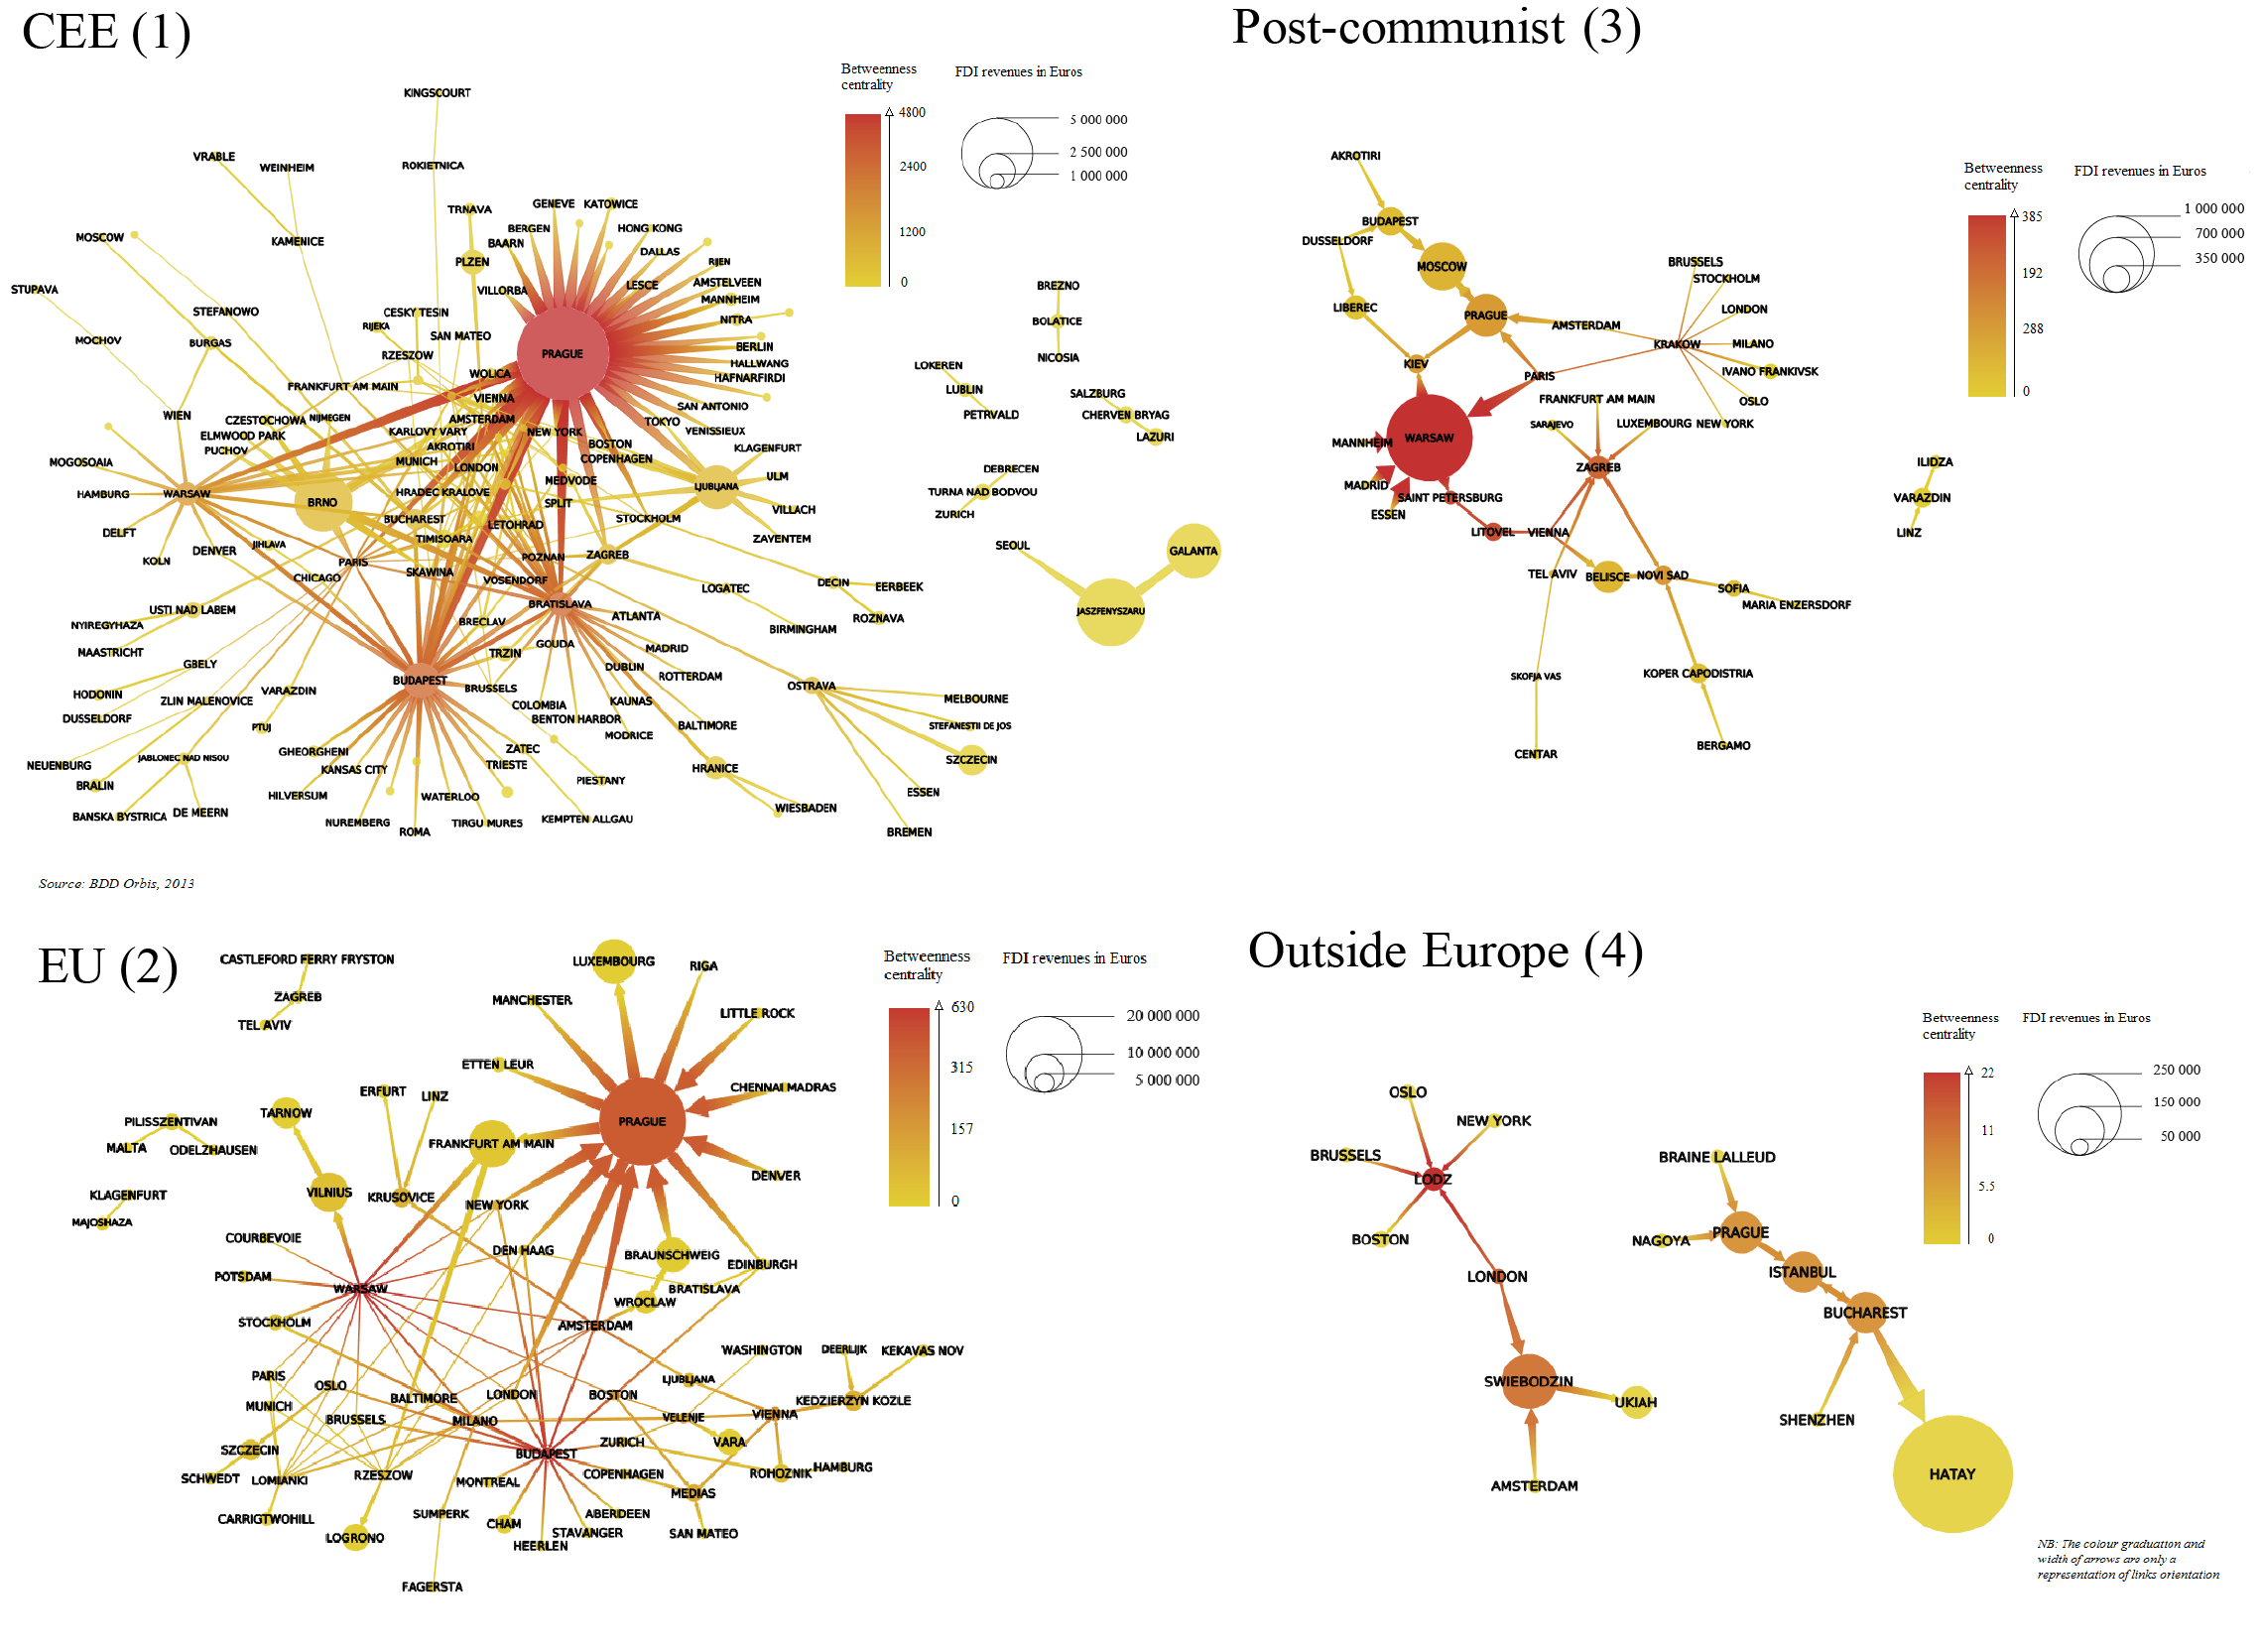
\includegraphics[width=0.7\textwidth]{figures/Figure1.png}
 \end{center}
 
  \textit{Central and Eastern European cities within ownership links of firms in 2013}

}

\sframe{Firm linkages structuring urban systems}{

 \begin{center}
 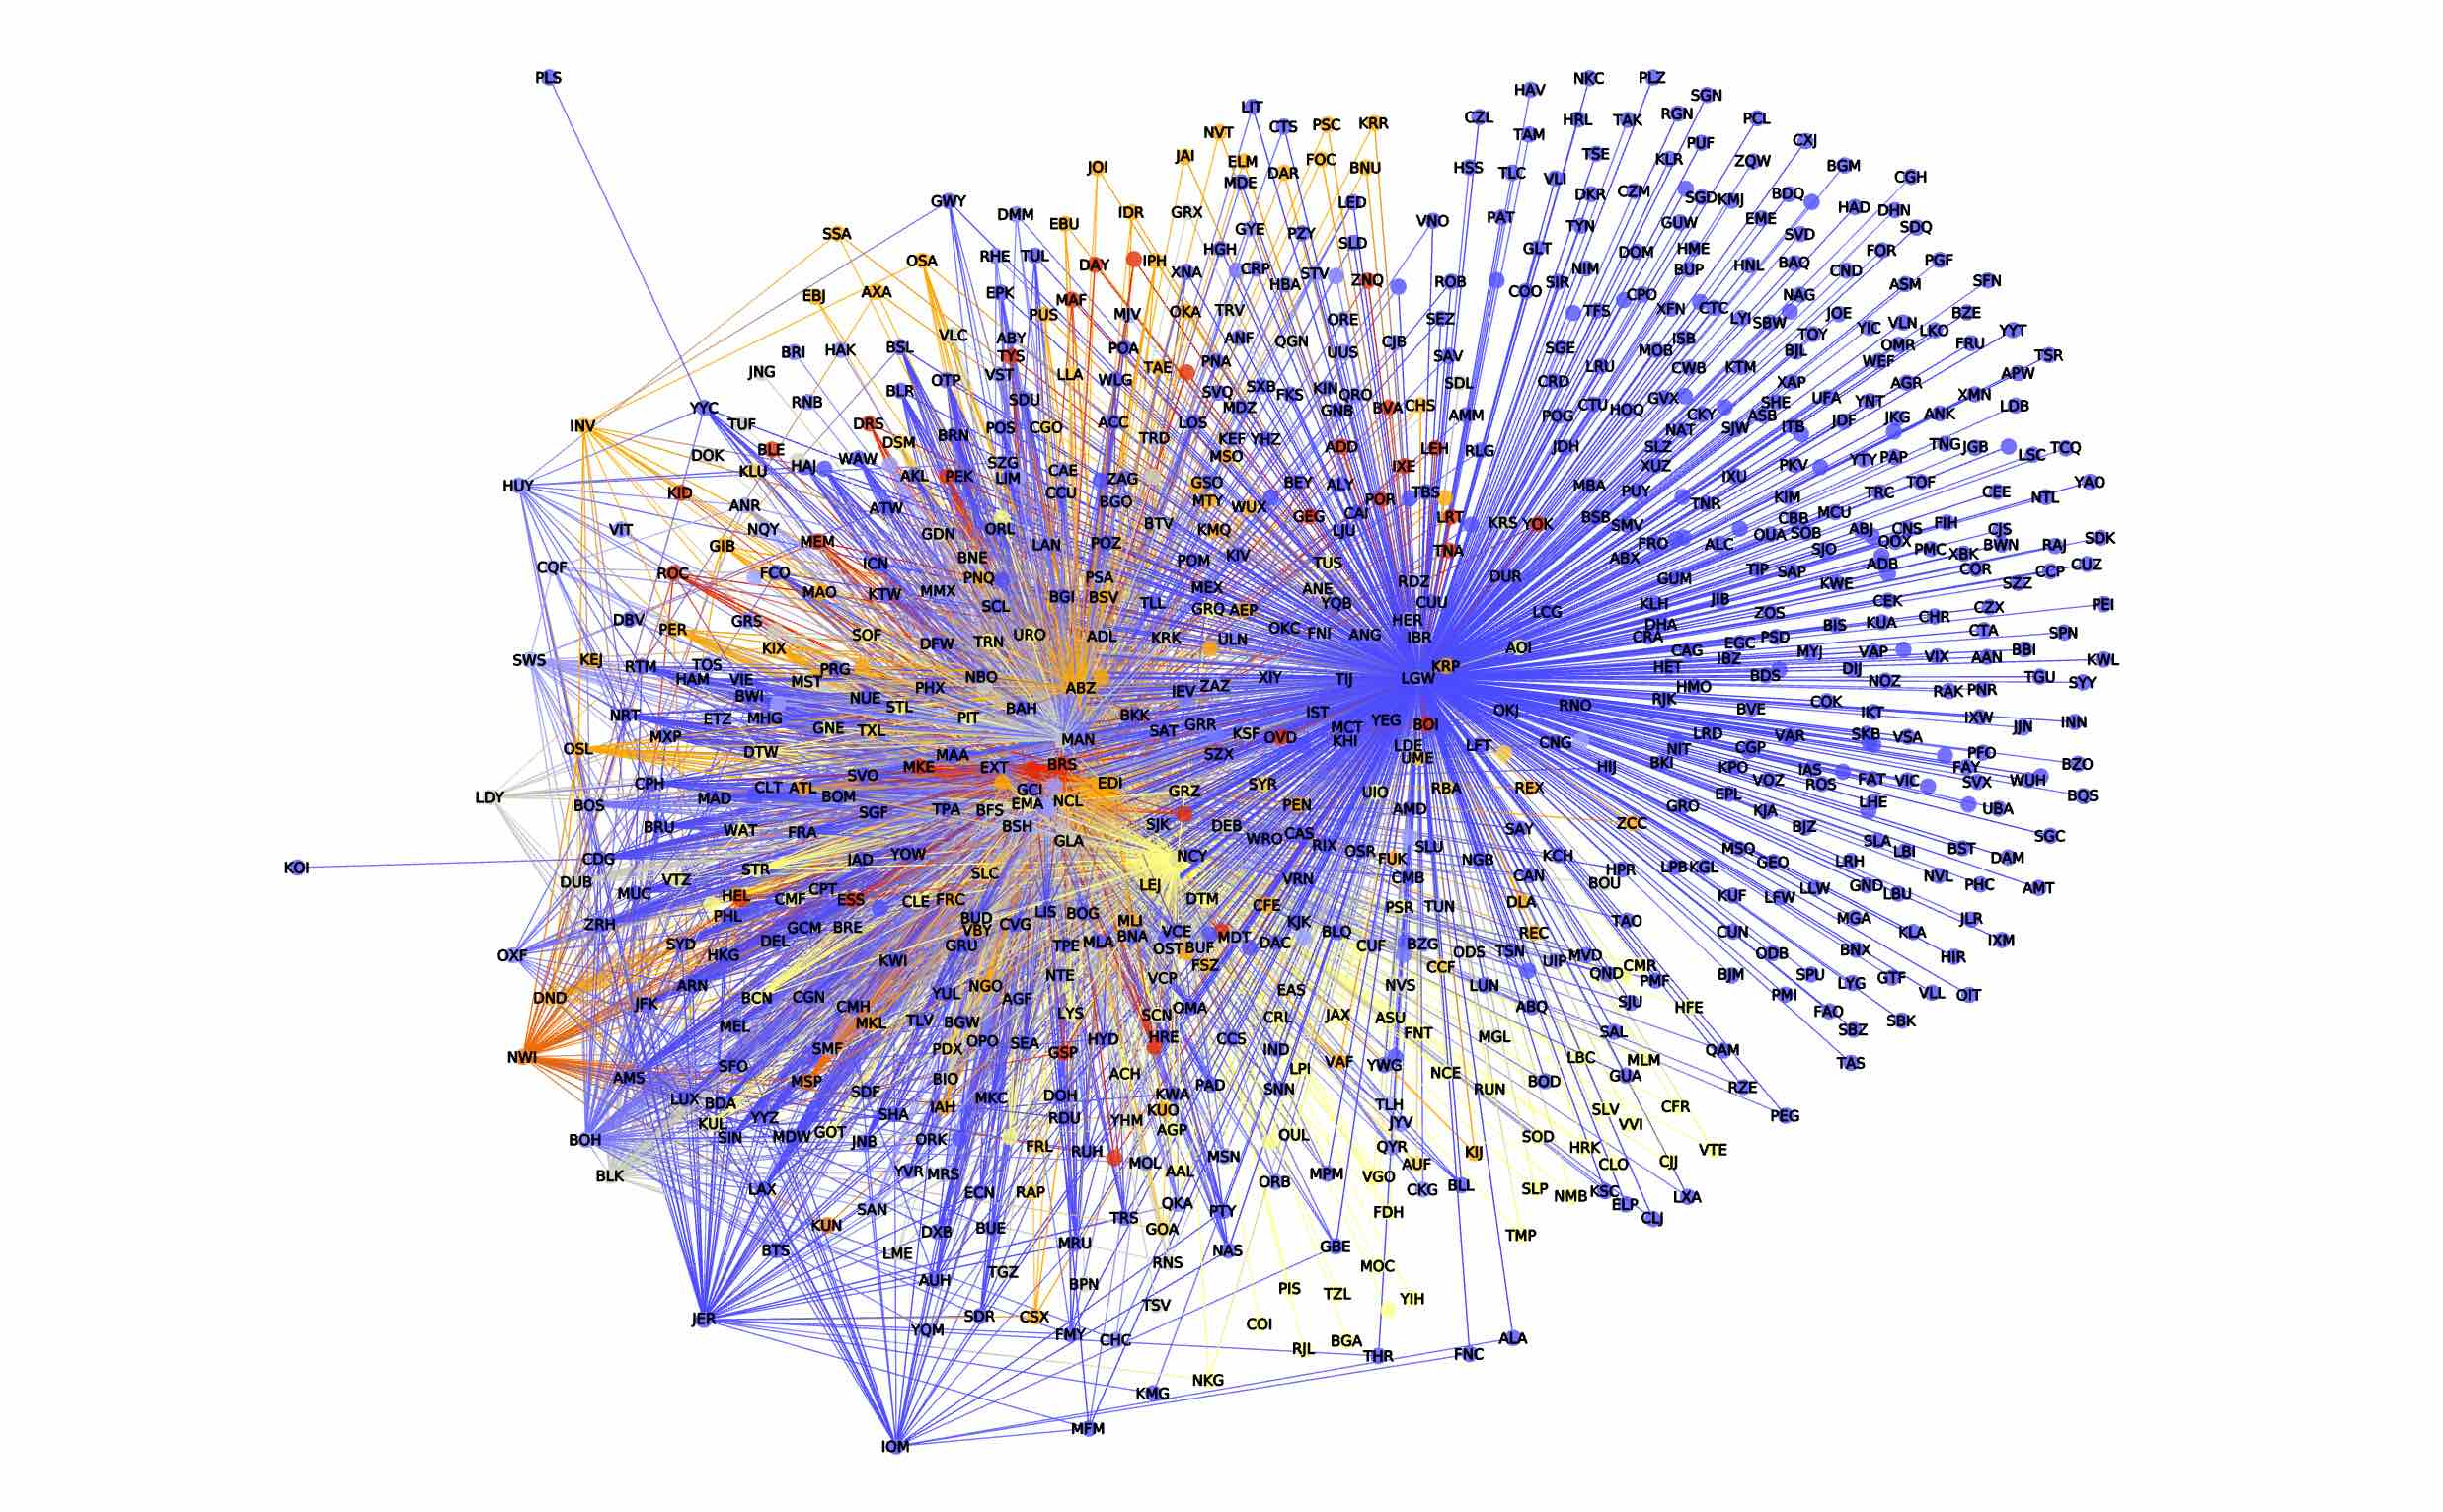
\includegraphics[width=0.7\textwidth]{figures/Figure2.png}
 \end{center}
 
  \textit{UK cities within transnational ownership links of firms in 2016}

}

% bon je ne sais pas si c'est utile mais au moins ca fait un exempple en plus (bon ok on ne voit rien)

\sframe{Urban firm linkages and geo-economic processes}{

Assumptions

\begin{itemize}
    \item Metropolisation vs. regionalisation effects
    \item Relationship local/global of multinational firm linkages 
    \item Specialisation-driven factors and drivers of innovation
    \item Macroeconomic exogenous chocs and resilience of urban systems 
\end{itemize}

\bigskip

$\rightarrow$ \textit{How can we capture geographical and economic processes within urban networks of firms with a generative model?}

\begin{itemize}
	\item Indirect inference on processes
	\item Includes path-dependency
\end{itemize}


}




\section{Model}

\sframe{Model rationale}{

$\rightarrow$ Cities are defined by their GDP and their profile regarding the proportion of firms in the different sectors. Links between cities are created in an iterative way, taking into account:

\medskip

    \begin{itemize}
        \item geographical proximity (distance or effective accessibility)
        \item geopolitical proximity (belonging to the same country or single market $\rightarrow$ application to Brexit)
        \item city size (economic size as GDP) 
        \item economic similarity (e.g. cosine distance between sector proximity as done in \cite{2019arXiv190505106C}
        \item previous linkages 
    \end{itemize}

% j'ai mis ca plus pour moi,enfin pour moi c'est plus clair pour la presentation
%  => oui c'est exactement ce quil fallait mettre !
% question a la con, mais est-ce que ce n'est pas tautolgique de dire que les villes et les liens sont definis par le GDP, ou le lien est bien defini par le GDP des noeuds.
}


\sframe{Formalization}{

Cities characterized by economic size $E_i$ (GDP) and economic structure $S_{ik}$ (probability distribution of firms within $K$ sectors)

% excuses-moi, mais je vais commencer a partir de la a te demander de m'expliquer, ca va te paraitre evident je suis desolee, mais c'est pour que je ne trompe pas en presentant
% a quoi correspond le i et j? En gros c'est ville i, puis la ville j? Le k c'est bien le nombre de secteurs? 
% -> oui exactement



\bigskip

Starting from an initial network, at each time step:
\begin{enumerate}
    \item Evolve city sizes $E_i \left(t \textrm{ + } 1 \right) \textrm{ = } f\left(E_j\left(t\right)\right)$ with an interaction model (\cite{raimbault2018indirect} or \cite{cottineau2015growing})
    % ici le = n'apparait pas dans la formule. le t c'est bien le temps?
    %  => oui t est le temps ; les = et + et ( ) qui passent pas c'est la template ucl, j'arrive pas a fixer alors il faut passer par le reswitch en mode texte
    \item Add a fixed number of links randomly, following a probability function of sizes, sector proximity, and geographical and socio-cultural proximity
\end{enumerate}

}


\sframe{Formalization}{

Probability for a new link follows a generalized Cobb-Douglas function

\medskip

\[
     p_{ij} \propto \left(\frac{E_{i}}{E}\right)^{\gamma_F} \cdot \left(\frac{E_{j}}{E}\right)^{\gamma_T} \cdot \left(\frac{w_{ij}}{W}\right)^{\gamma_W} \cdot s\left(S_{ik},S_{jk}\right)^{\gamma_S} \cdot \exp \left(- \gamma_G \cdot d_{ij}\right) \cdot \exp \left(- \gamma_D \cdot g_{ij}\right)
\]

% idem ici, pij c'est la probabilite d'un lien entre i et j oui?
%. => oui, sachant qu'il y a un nouveau lien (il y en a un par pas de temps), la proba qu'il soit entre i et j
% les gamma c'est les parametres du modele et Ei c'est le gdp de la ville et pourquoi c'est sur E, ca vient de la formule du modele gravitaire oui?
% oui c'est les parametres de Cobb douglas qui permettent d'ajuster l'importance relative entre chacun des facteurs, et la maniere dont ils influencent (en gros gamma << 1 favorise majoritairmenent les faibles avleurs, gamma = 1 lineaire, gamma >> 1 favorise les fortes valeurs
<<<<<<< HEAD
% le modele gravitaire c'est des masses m_i m_j / d_{ij} mais il y a toujours un facteur de normalistaion qu'il faut determiner ou non (selon que c'est avec ocntraintes - c'est lien a ce que fait Robin Morphet s'il t'en a deja parl�) - dans notre cas c'est la cobbdouglas qui doit avoir ses variables dans 0,1, donc on normalise comme la part du gdp total
% Wij c'est quoi? il me semble que tu as dit que c'est le lien du passé e
=======
% le modele gravitaire c'est des masses m_i m_j / d_{ij} mais il y a toujours un facteur de normalistaion qu'il faut determiner ou non (selon que c'est avec ocntraintes - c'est lien a ce que fait Robin Morphet s'il t'en a deja parlé) - dans notre cas c'est la cobbdouglas qui doit avoir ses variables dans 0,1, donc on normalise comme la part du gdp total
% Wij c'est quoi? il me semble que tu as dit que c'est le lien du passé e
>>>>>>> 6da27f247dc6a5859125a5d7c204c2c4deef99e0
% oui c'est le poids du lien precedennt
% Sik c'est la structure economique defini par le cosine similarity 
% => la fonction s donne la cosine similarity entre S_{ik} et S_{jk} les structures industrielles
% comment est definie le gij donc la distance socio-culturelle?
% => pour l'instant c'est la distance entre les centroides des pays correspondants (c'est un trick pour le systeme synthetique, pour une application sur donnees reelles faudra faire des modeles stat avec effets fixes pour l'estimer)

\medskip

where $E \textrm{ = } \sum_k E_k$, $W \textrm{ = } \sum_{i,j} w_{ij}$, $s$ is a proximity measure given by cosine similarity, $d_{ij}$ euclidian distance, and $g_{ij}$ a socio-cultural distance

\bigskip
\bigskip

\textbf{Model parameters: } $\gamma_F, \gamma_T, \gamma_W, \gamma_S, \gamma_D \textrm{ = } \frac{1}{d_G}, \gamma_G \textrm{ = } \frac{1}{d_G}$

}

\sframe{Model indicators}{

\textbf{Geographical indicators:}

\begin{itemize}
    \item Internationalisation (modularity of countries in the network)
    \item Metropolisation (correlation between weighted degree and city size)
    \item Regionalisation (correlation between length and flow of links, stratified by size of extremities)
    \item Specialisation (correlation between sector proximity and flow of links, stratified by size of extremities)
\end{itemize}

\bigskip

\textbf{Network and flows indicators:}

%  networkModularity, networkAvgCommunitySize, networkDegreeHierarchy, networkAvgDegree, networkDegreeEntropy, flowsHierarchy, flowsEntropy, rhoDegreeSize, rhoFlowDistancePos, rhoFlowDistance

\begin{itemize}
    \item Louvain modularity, community sizes
    \item Degree and flows distribution (average, hierarchy, entropy)
    \item Correlations (degree-size, flow-distance)
\end{itemize}

}

\sframe{Simulation on synthetic systems of cities}{

% la ou avant il faut surement expliquer que c'est pas totalement synthetique, que tu pars de X villes europeennes de plus de 50 000 habitants (pour les plus nuls comme moi)
% si c'est completement synthetiques, l'histoire des villes europeenes c'est pour avoir les ordres de grandeur de la hierarchie et du nombre de villes, mais c'est pas parametrise sur des vraies donnees - mais oui ca ca sera explique dans comment construire le systeme de ville synthetique.

% ok desolee je n'avais pas bien compris 
% javais mal explique ^-^
 
\justify
 
\textit{Following \cite{raimbault2018space}, geosimulation models must be studied within synthetic controllable urban contexts in order to (i) understand intrinsic behavior of the model and robust qualitative stylized facts; (ii) study the sensitivity to the spatial configuration}

\bigskip

Generation of a continent-scale urban system with stylized order of magnitude corresponding to Europe:

\medskip

\footnotesize

\begin{enumerate}
    \item Generate $N \textrm{ = } 700$ cities with size following a power law $E_i \textrm{ = } E_0 \cdot i^{-\alpha}$ with $E_0 \textrm{ = } 10^{11}$ and $\alpha \textrm{ = } 1.1$ (computed on Europe for GDP with cities larger than 50.000 inhabitants)
    \item Distribute them randomly in space (\cite{simini2019testing} vs \cite{banos2011christaller})
    \item Create countries with k-means clustering ($C \textrm{ = } 30$)
    \item Distribute sectors such that (i) smaller cities are more specialized and (ii) larger cities are more knowledge-based, with a one dimensional axis to position sectors $1/K \ldots 1$ where the density $f\left(k\right)$ follows a log-normal with $\left(\mu,\sigma\right)$ such that $\sqrt{\Var f} \textrm{ = } K/2$ for the largest, $\sqrt{\Var f} \textrm{ = } 1/K$ for the smallest
\end{enumerate}

 
}

\section{Results}

\sframe{Implementation and experiments}{

\textbf{Implementation}

\begin{itemize}
	\item Model implemented in NetLogo (good compromise interactivity / ergonomy), with fast data structures (matrix/table extensions)
	\item Integrated seamlessly into OpenMOLE \cite{reuillon2013openmole} for model exploration (NetLogoTask)
\end{itemize}


\medskip

\textbf{Experiments}

% for now no dynamics of cities

\begin{itemize}
	\item Current experiment: only network dynamics (short time scale)
	\item One-factor sampling with 100 repetitions to assess statistical properties (good convergence, average sharpe ratios for indicators all larger than 5)
	\item Grid sampling with 20 repetitions for model behavior %(2years 5months of computation)
\end{itemize}

}

\sframe{Simulation of urban networks}{
    
    % examples
    
    \begin{center}
    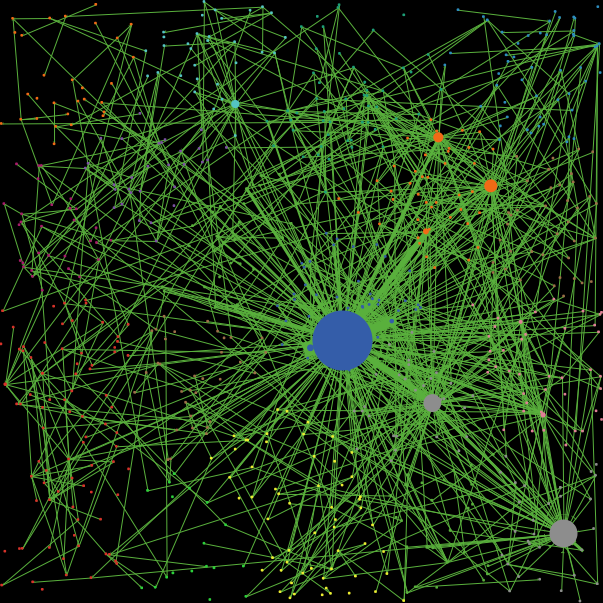
\includegraphics[width=0.48\textwidth]{figures/ex_alleq-highgravity_seed-12102_t1500.png}\hspace{0.1cm}
    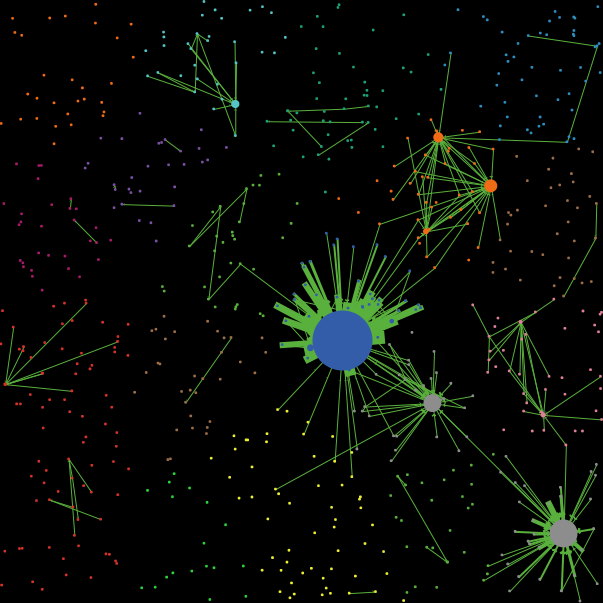
\includegraphics[width=0.48\textwidth]{figures/ex_alleq-lowgravity_seed-12102_t1500.png}
	\end{center}

	\medskip

	\textit{Networks at $t \textrm{ = } 1500$, for default parameters values and high gravity (left) and low gravity (right)}

}


%\sframe{Statistical convergence}{

%$\rightarrow$ Good convergence for most indicators: average sharpes ratios on a one-factor sampling above 5 (except for metropolization index $\simeq 1.5$)

% + histograms

%\bigskip
%}


\sframe{Effect of interaction decay}{
    
    % One factor sampling results
    %  20190924_162740_ONEFACTOR_REPLICATIONS_SYNTHETIC_GRID
    
    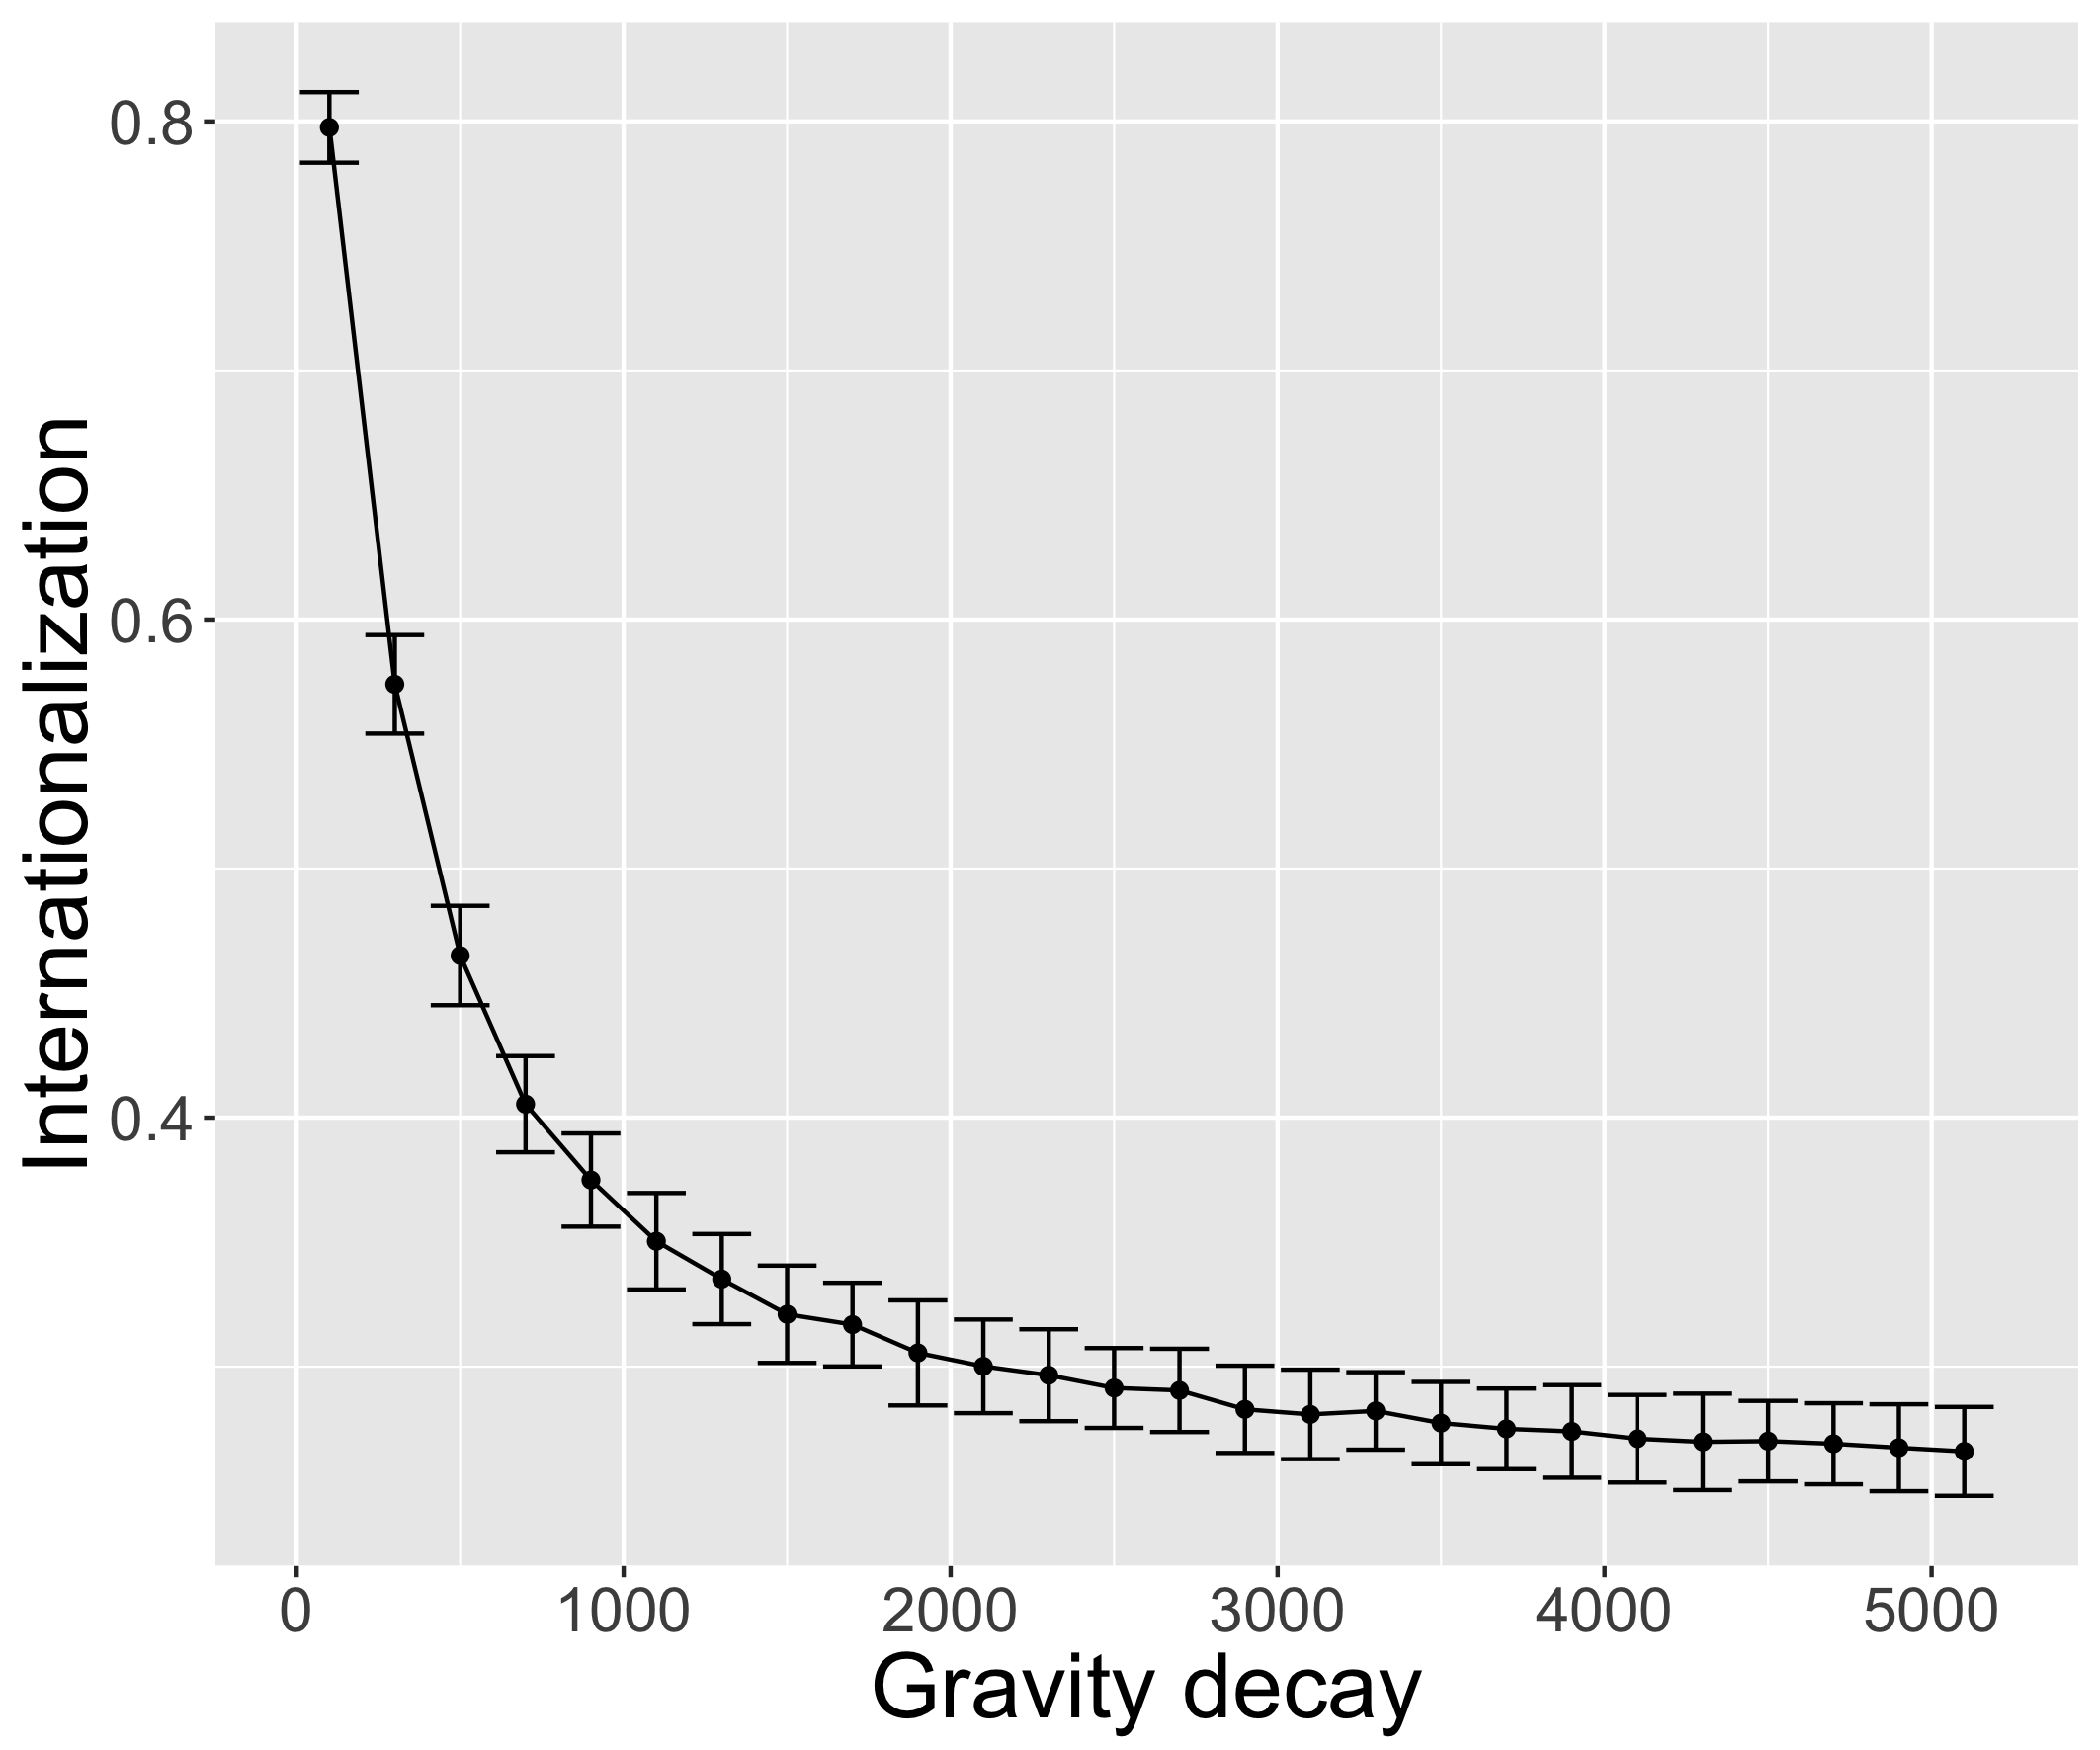
\includegraphics[width=0.48\textwidth]{figures/internationalization-gravityDecay_errorbars.png}
    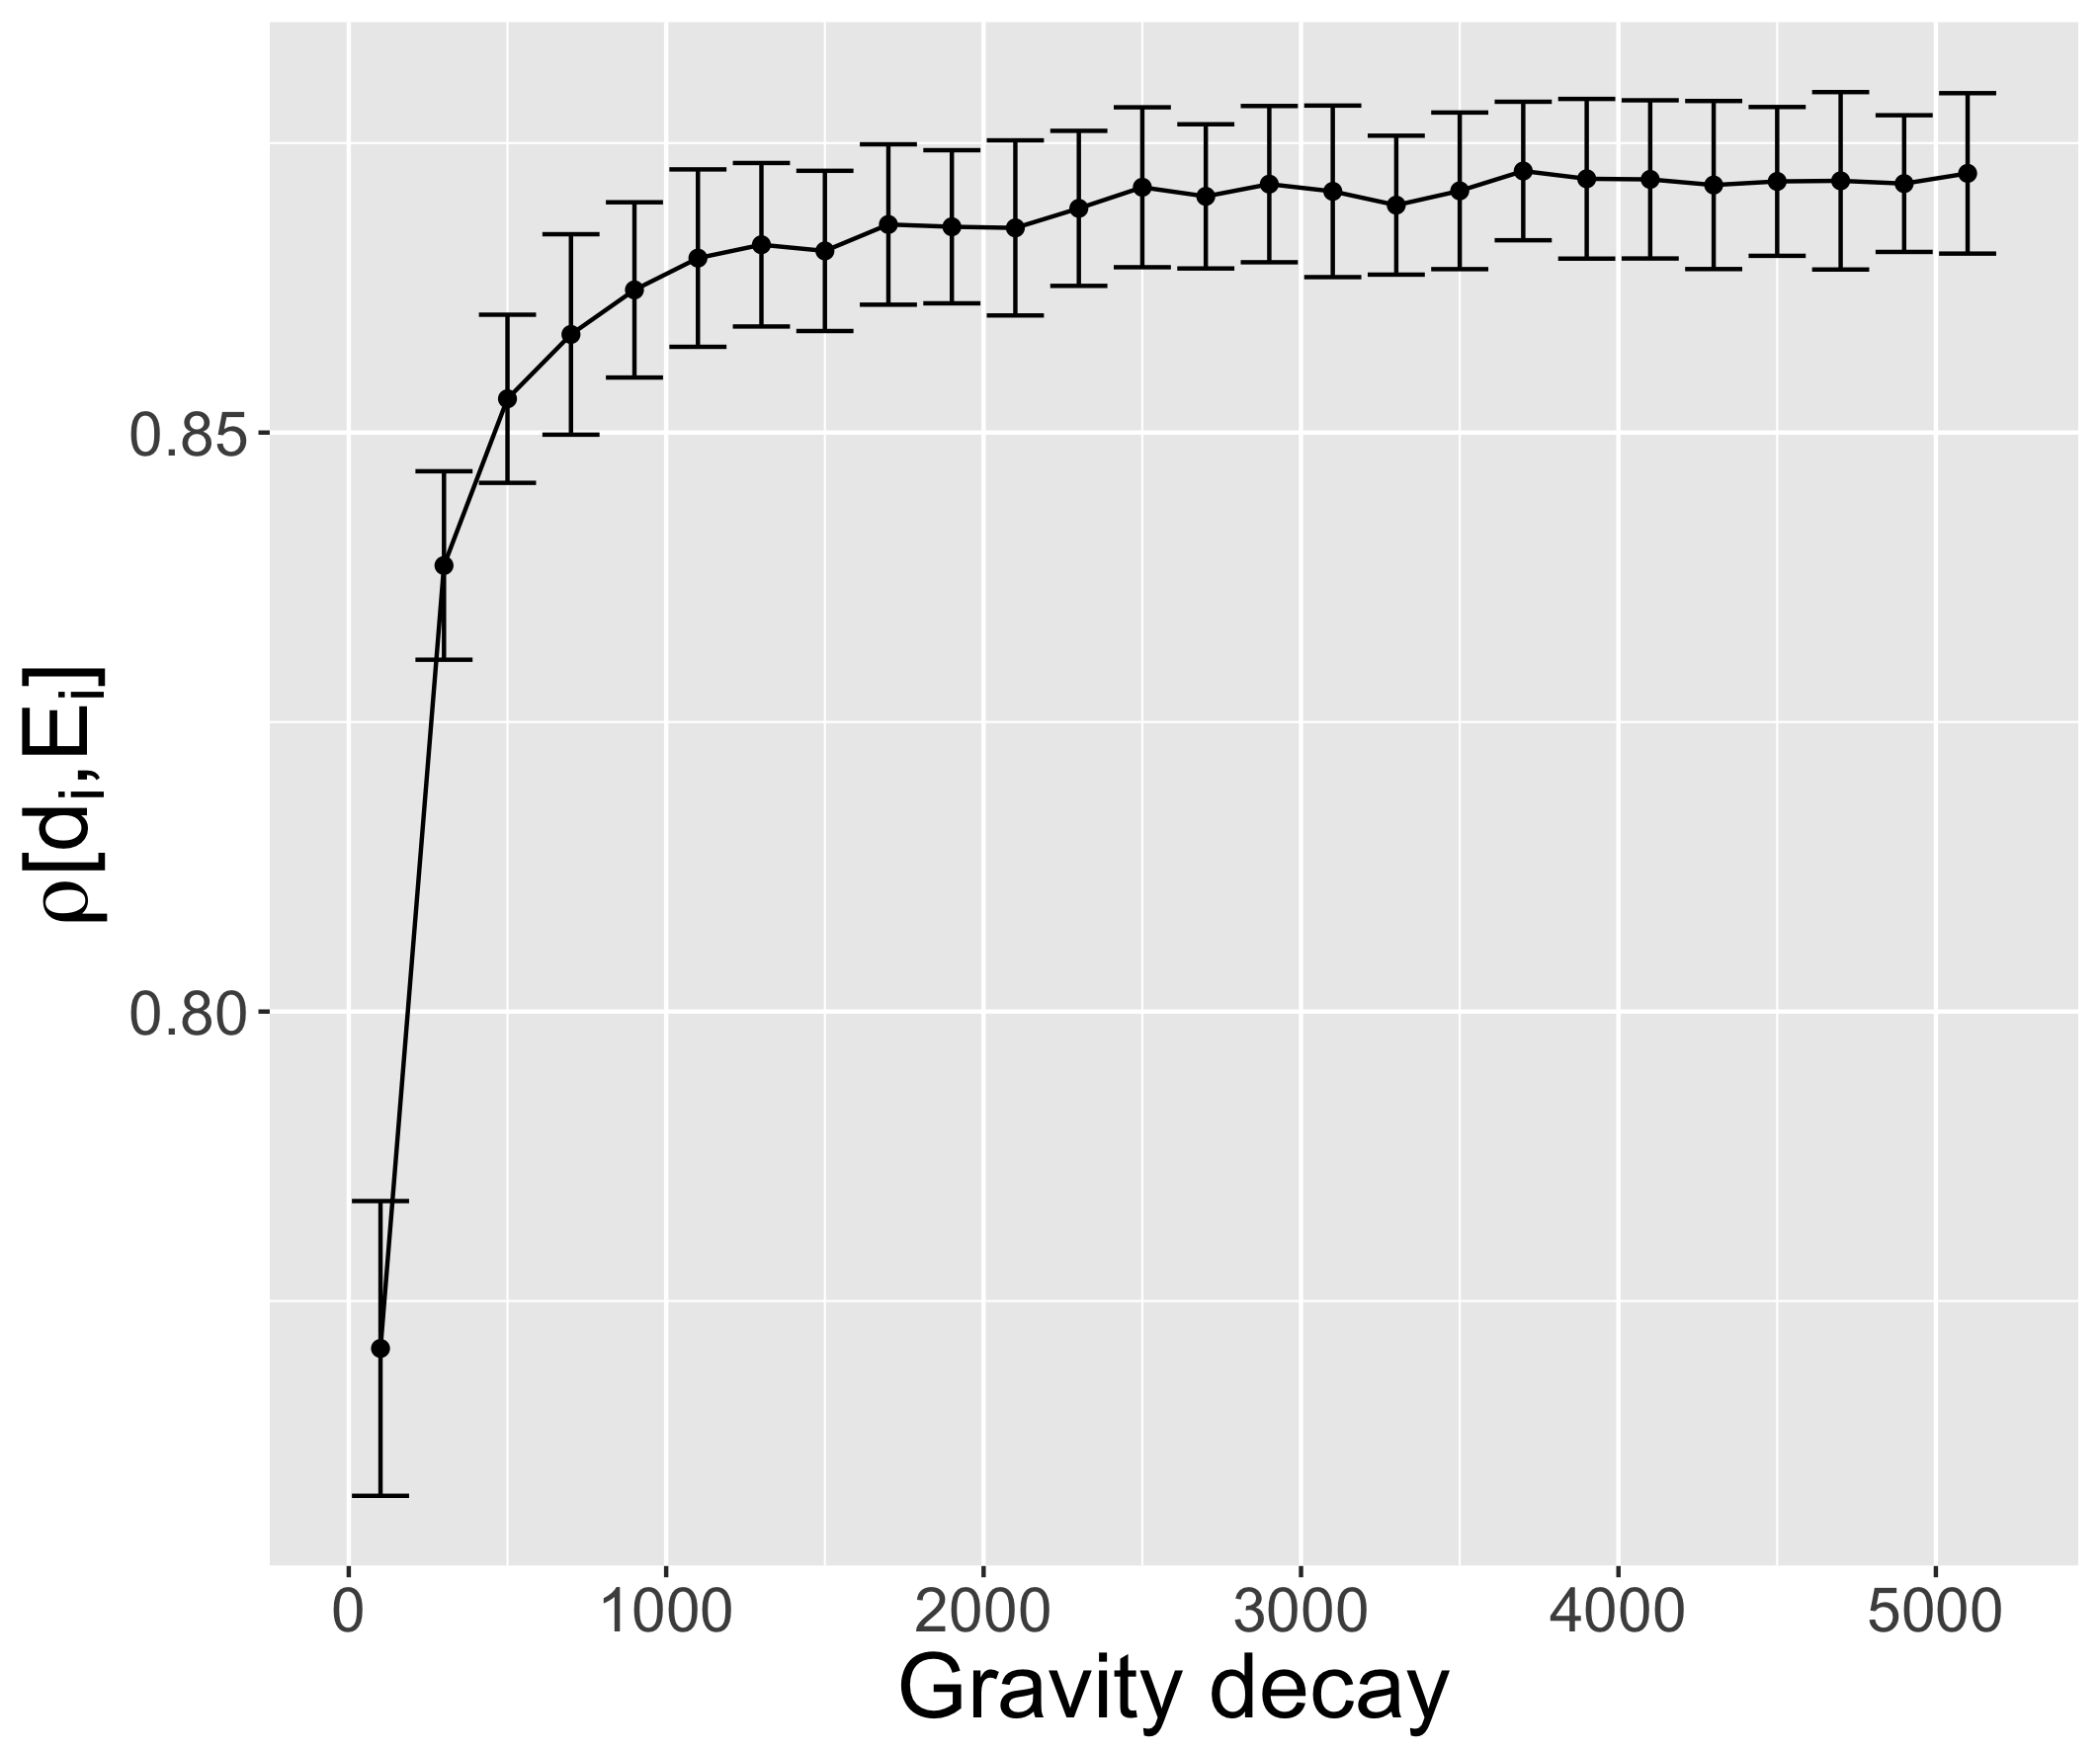
\includegraphics[width=0.48\textwidth]{figures/rhoDegreeSize-gravityDecay_errorbars.png}
    
    \medskip
    
    \footnotesize
    
    \textit{(Left) Internationalization index decreases exponentially with gravity decay; (Right) Correlation between city weighted degree and size. Both plots show a transition from a local to a global regime.}
    
}

% alors la je ne comprend pas desolee l'interpretation de l'evolution des courbes, l'internationalisation (qui est defini par la modularite diminue avec le temp?
% et le p(di,E) proba entre distance et poids economique? comment tu interpretes ca? il y a un seuil a la fin
% du coup je ne comprend pas bien comment interpreter
%  => c'est pas dans le temps, c'est en fonction du parametre de gravity ; internationalization comme c'est la modularite elle est minimisee plus c'est internataional

\sframe{Effect of sector proximity}{
    
    % One factor sampling results
    %  20190924_162740_ONEFACTOR_REPLICATIONS_SYNTHETIC_GRID
    
     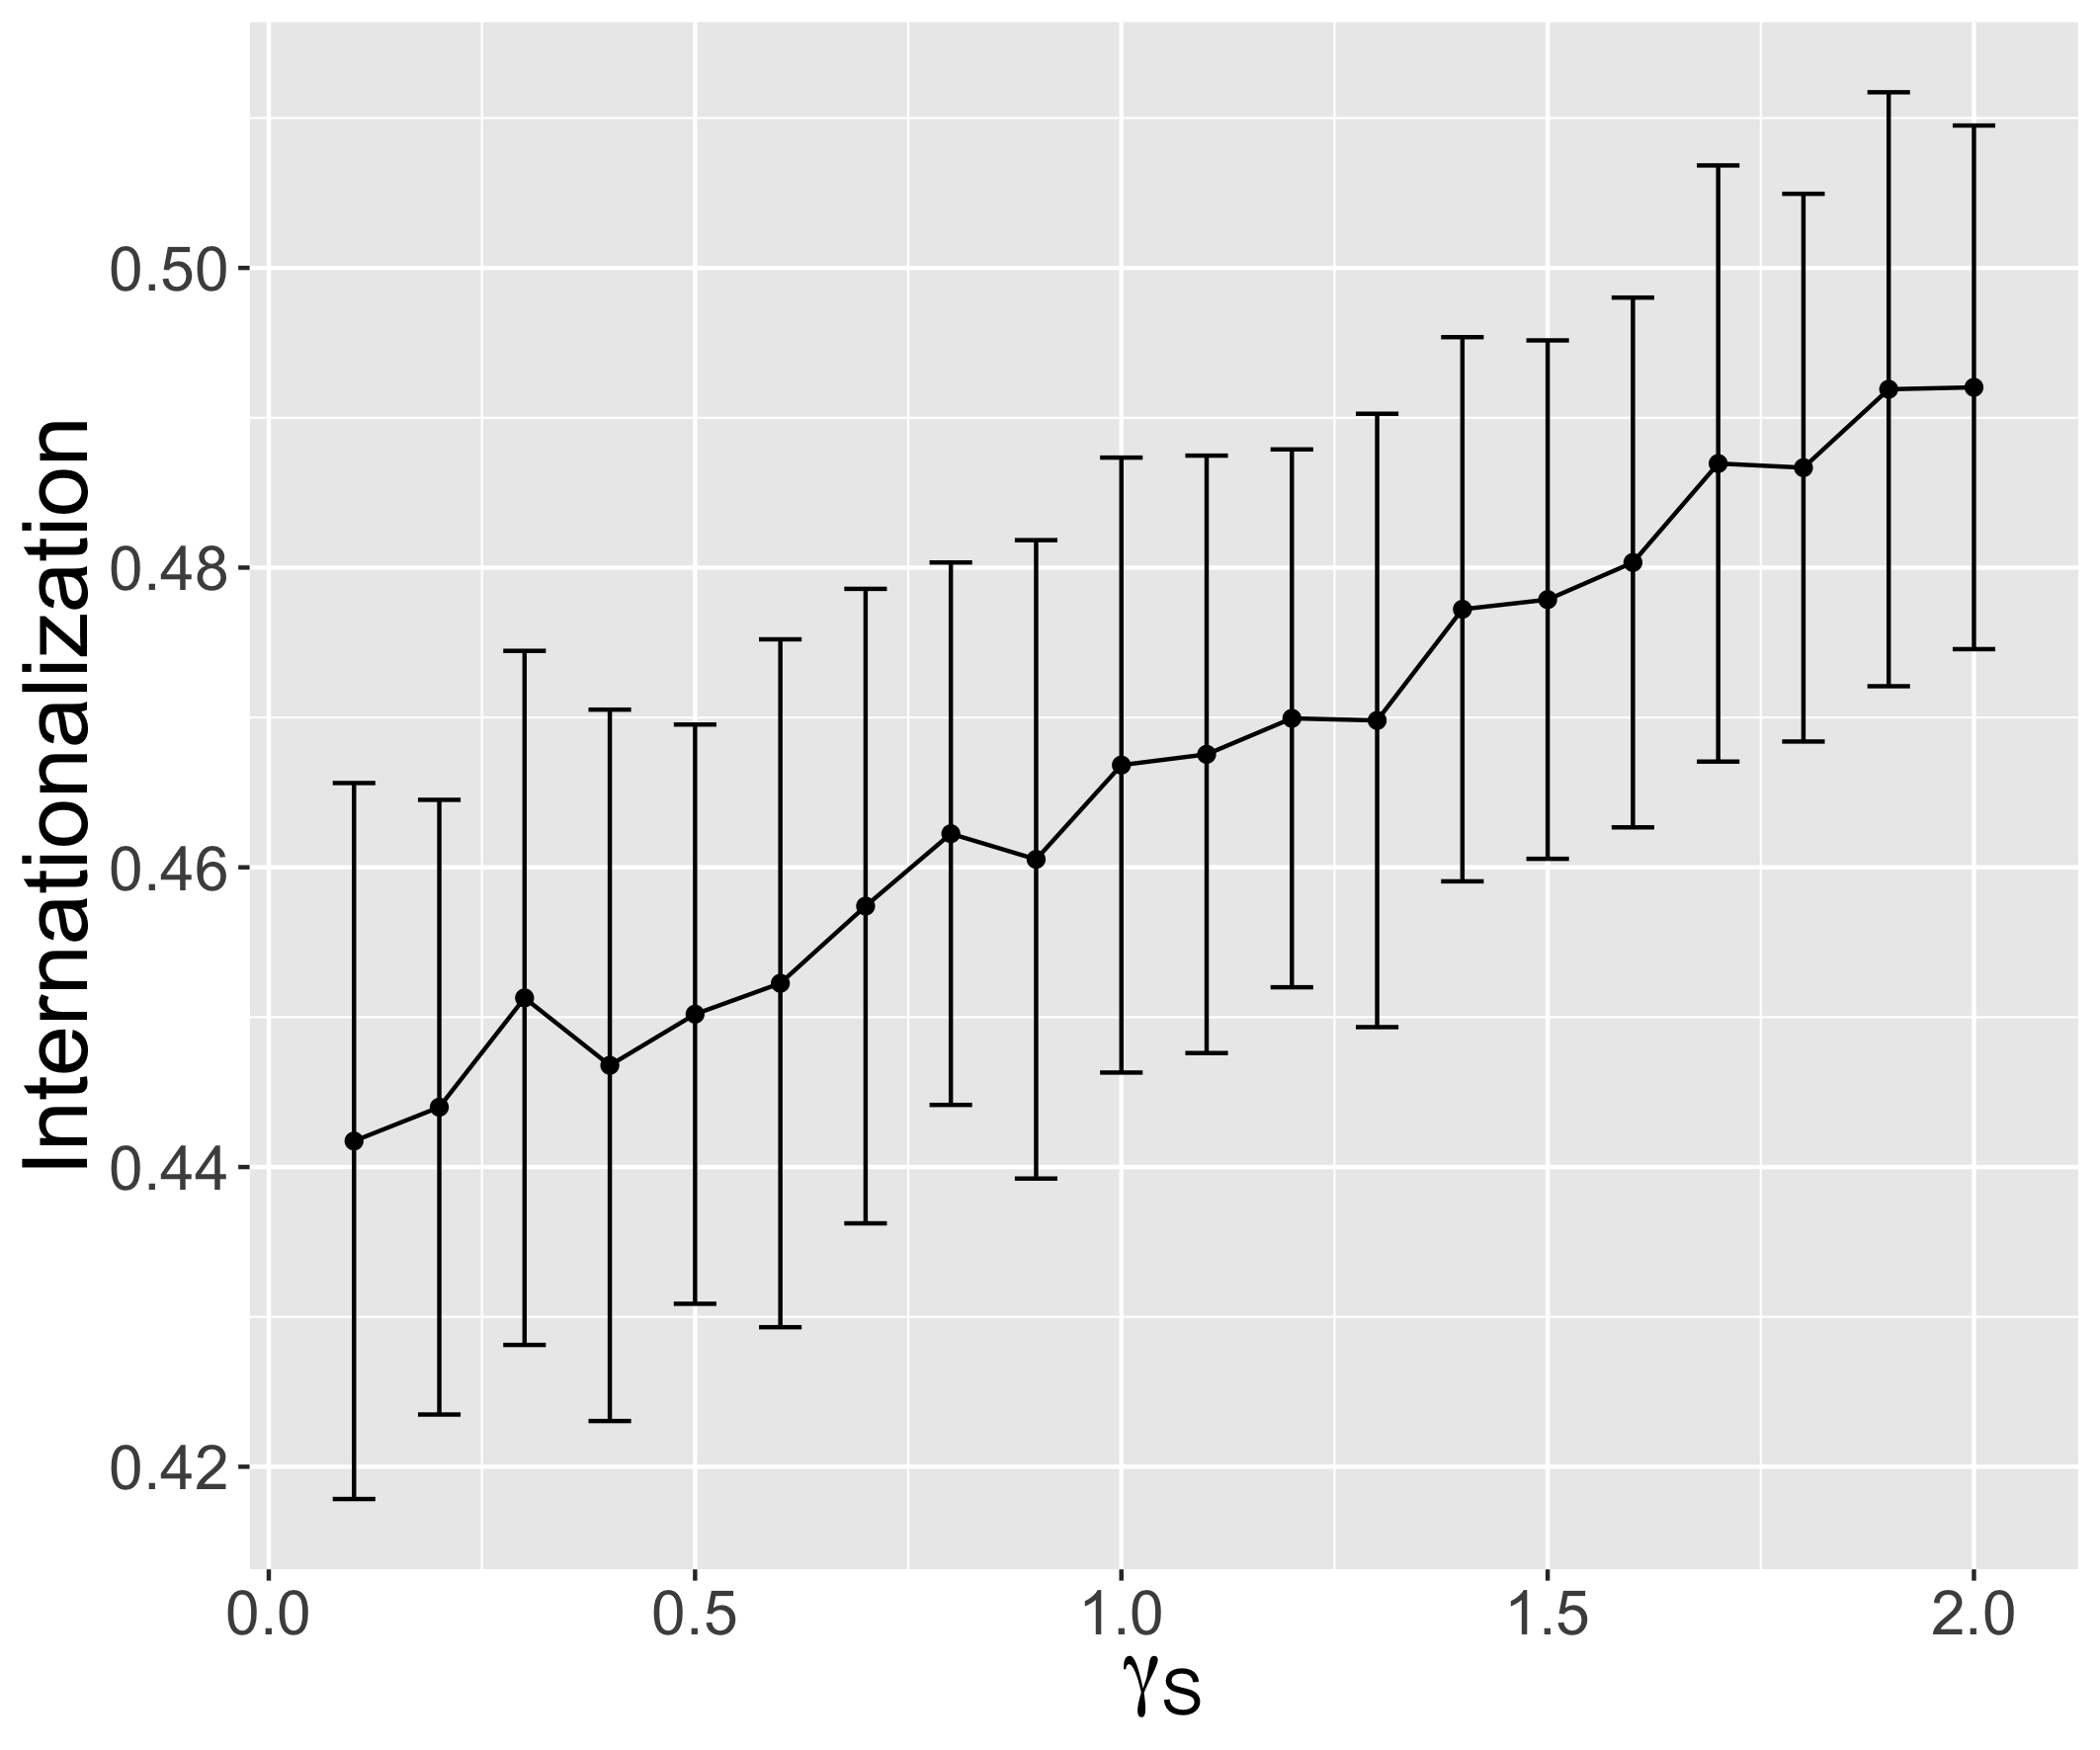
\includegraphics[width=0.48\textwidth]{figures/internationalization-gammaSectors_errorbars.png}
    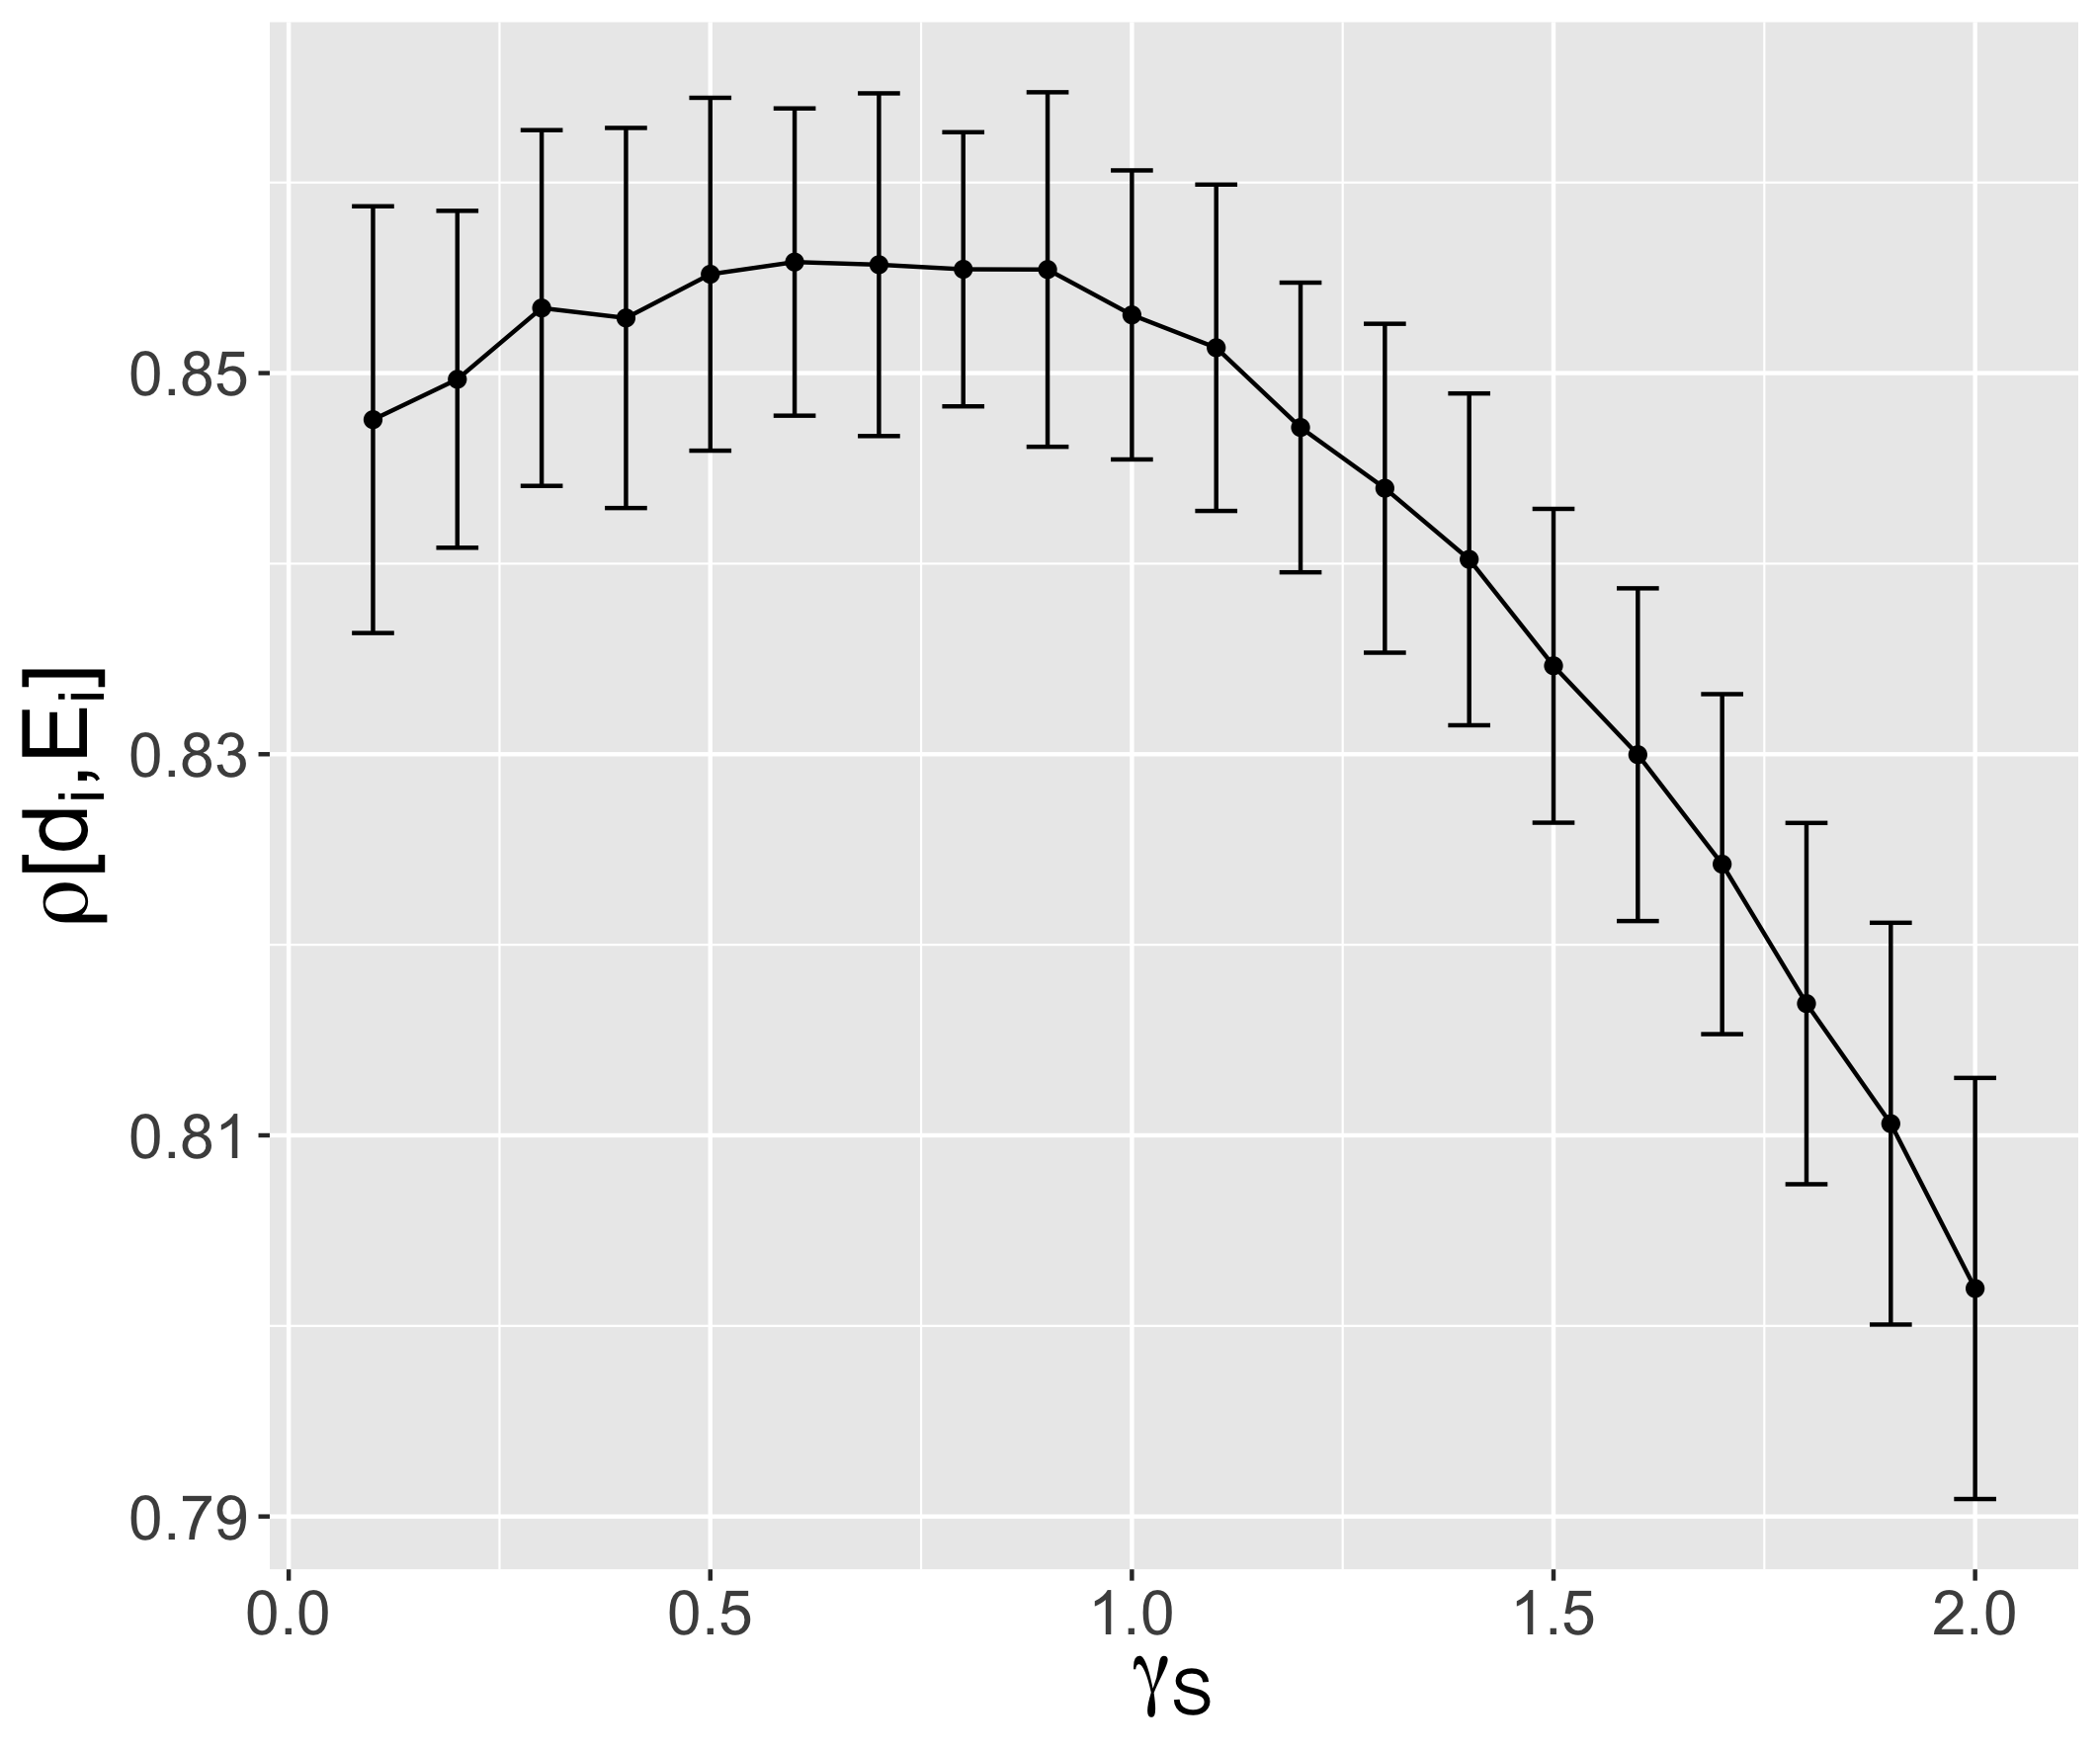
\includegraphics[width=0.48\textwidth]{figures/rhoDegreeSize-gammaSectors_errorbars.png}
    
    \medskip
    \footnotesize
    
    \textit{(Left) Internationalization varies linearly with sector proximity $\gamma_S$; (Right) Correlation between degree and size exhibits a maximum, witnessing an intermediate regime where size is the most important}
    
    
}


\sframe{Grid exploration: internationalization}{

    \centering

    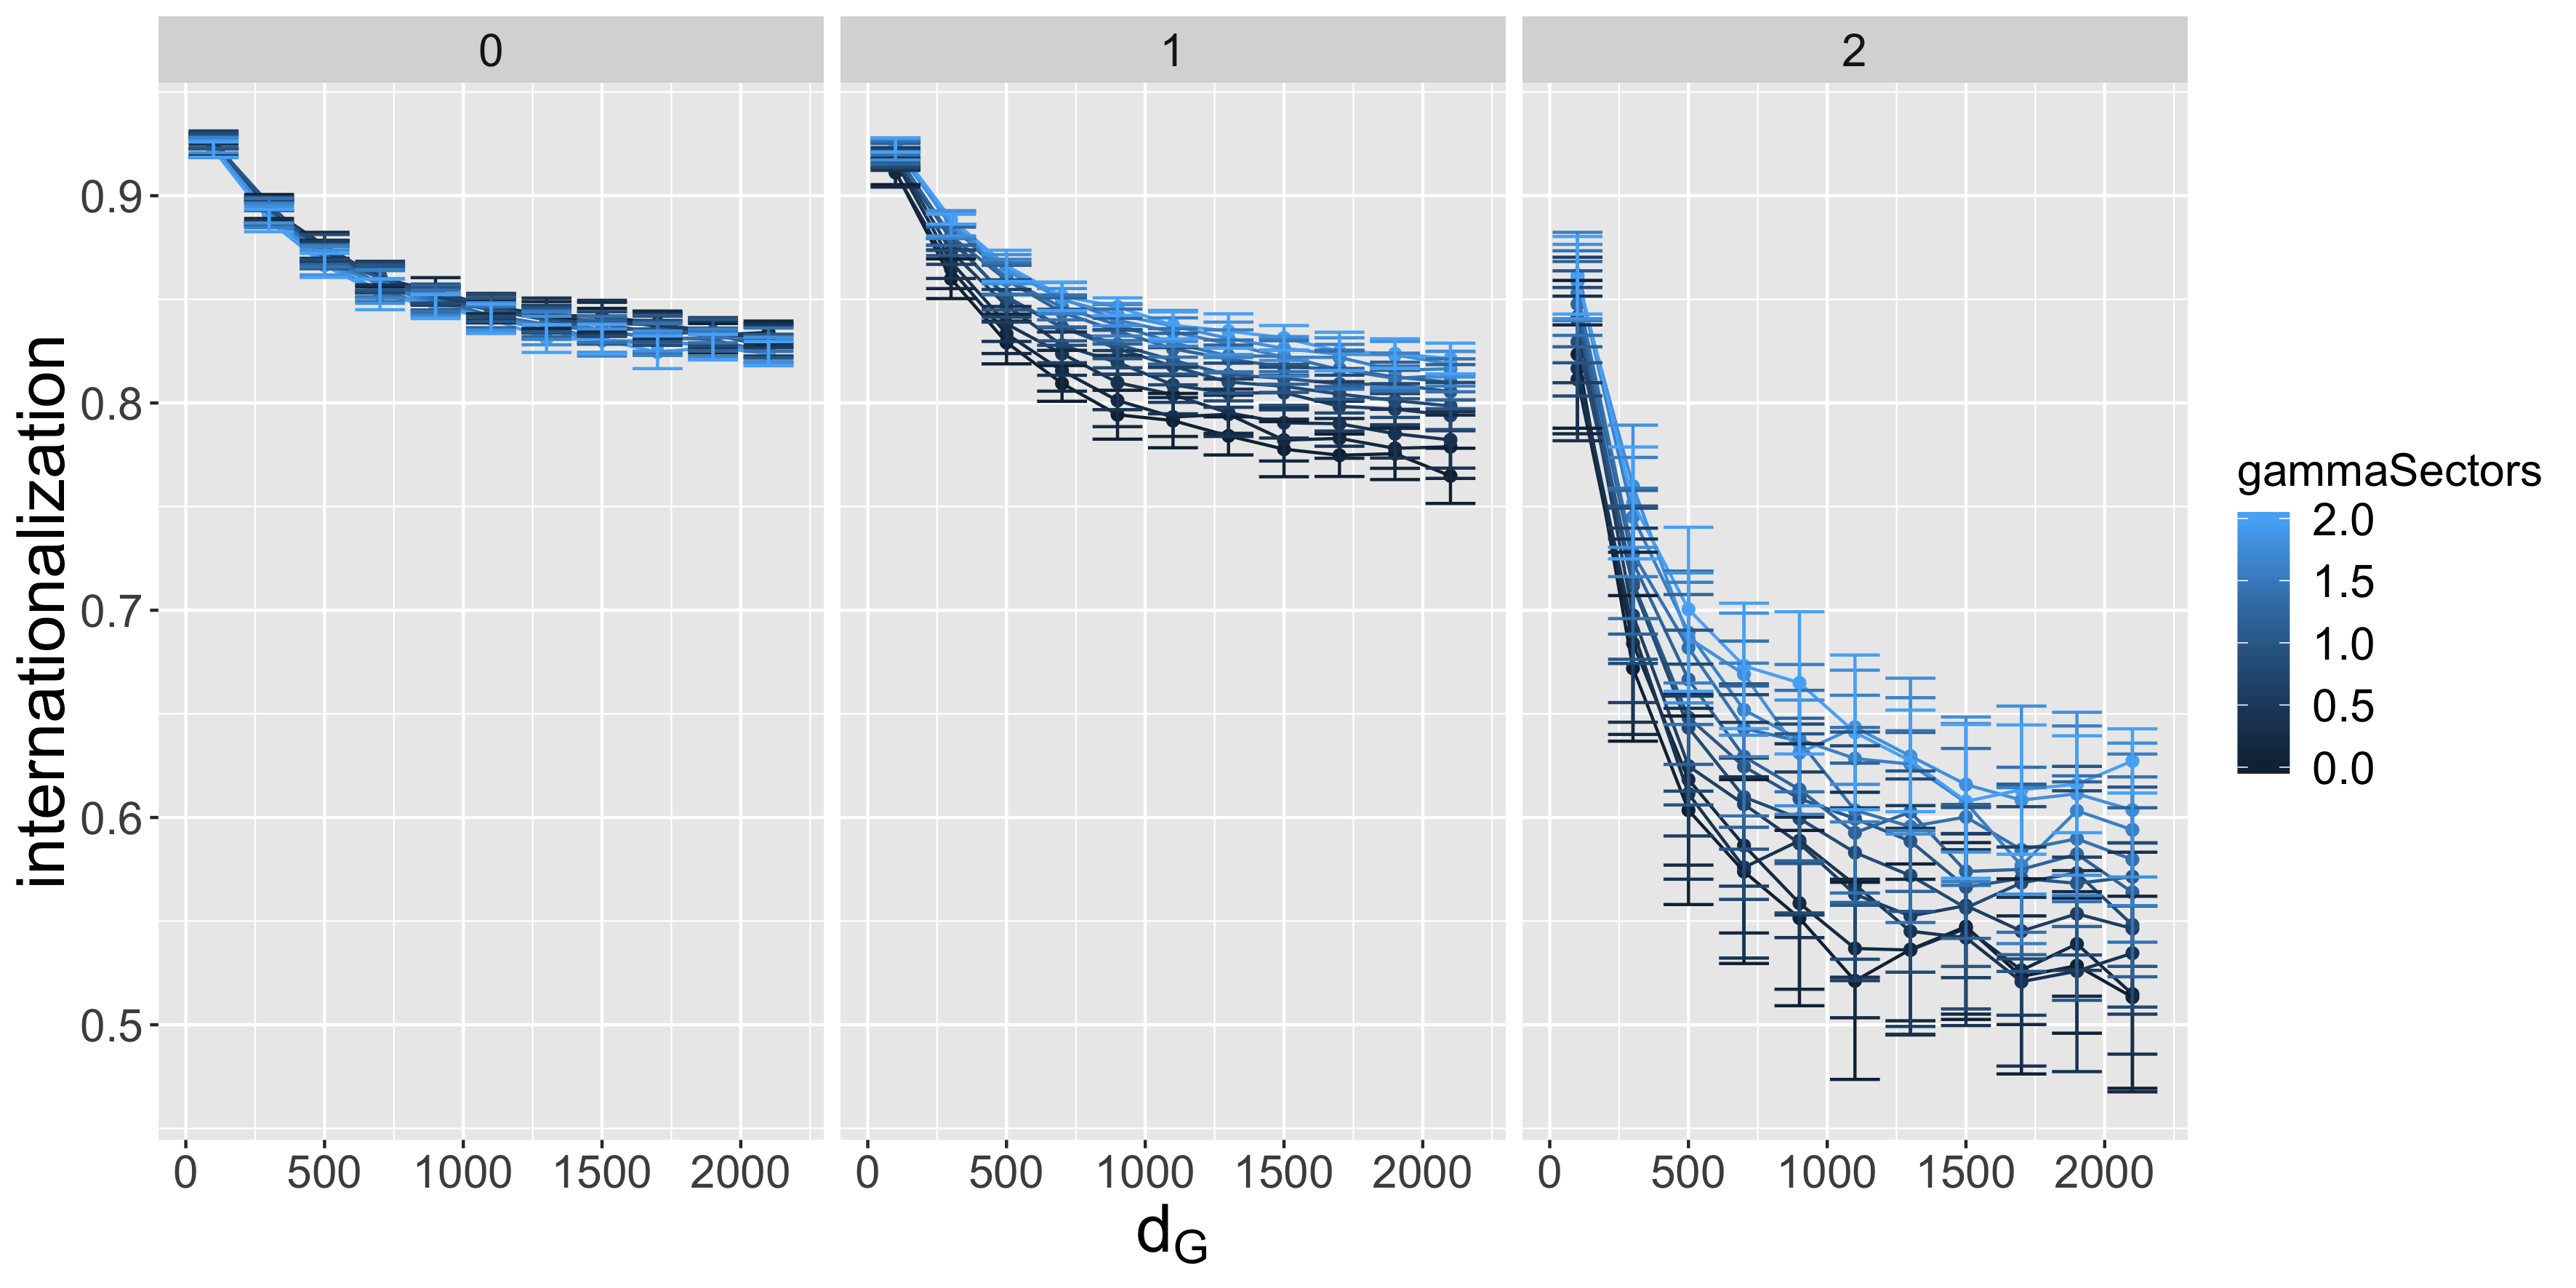
\includegraphics[width=\textwidth]{figures/internationalization_countryGravityDecay200_gammaDestination0_facetwrapgammaOrigin_colorgammaSectors.png}
    
    \medskip
    
    \footnotesize
    
    \textit{}
    
}

% alors tu as explique pendant la presentqtion pour Mike, mais je n'ai pas compris pourquoi il a trois graphiques 0 1 2 et pourquoi le 3 est si different:?
% je pense qu'il faut reconmmer en un truc plus clair l'axe des ordonnees et les 0, 1, 2
% dG c'est quoi, c'est toujours le pqs de temps? donc la meme chose que le gravity decay?

\sframe{Grid exploration}{

    \centering

    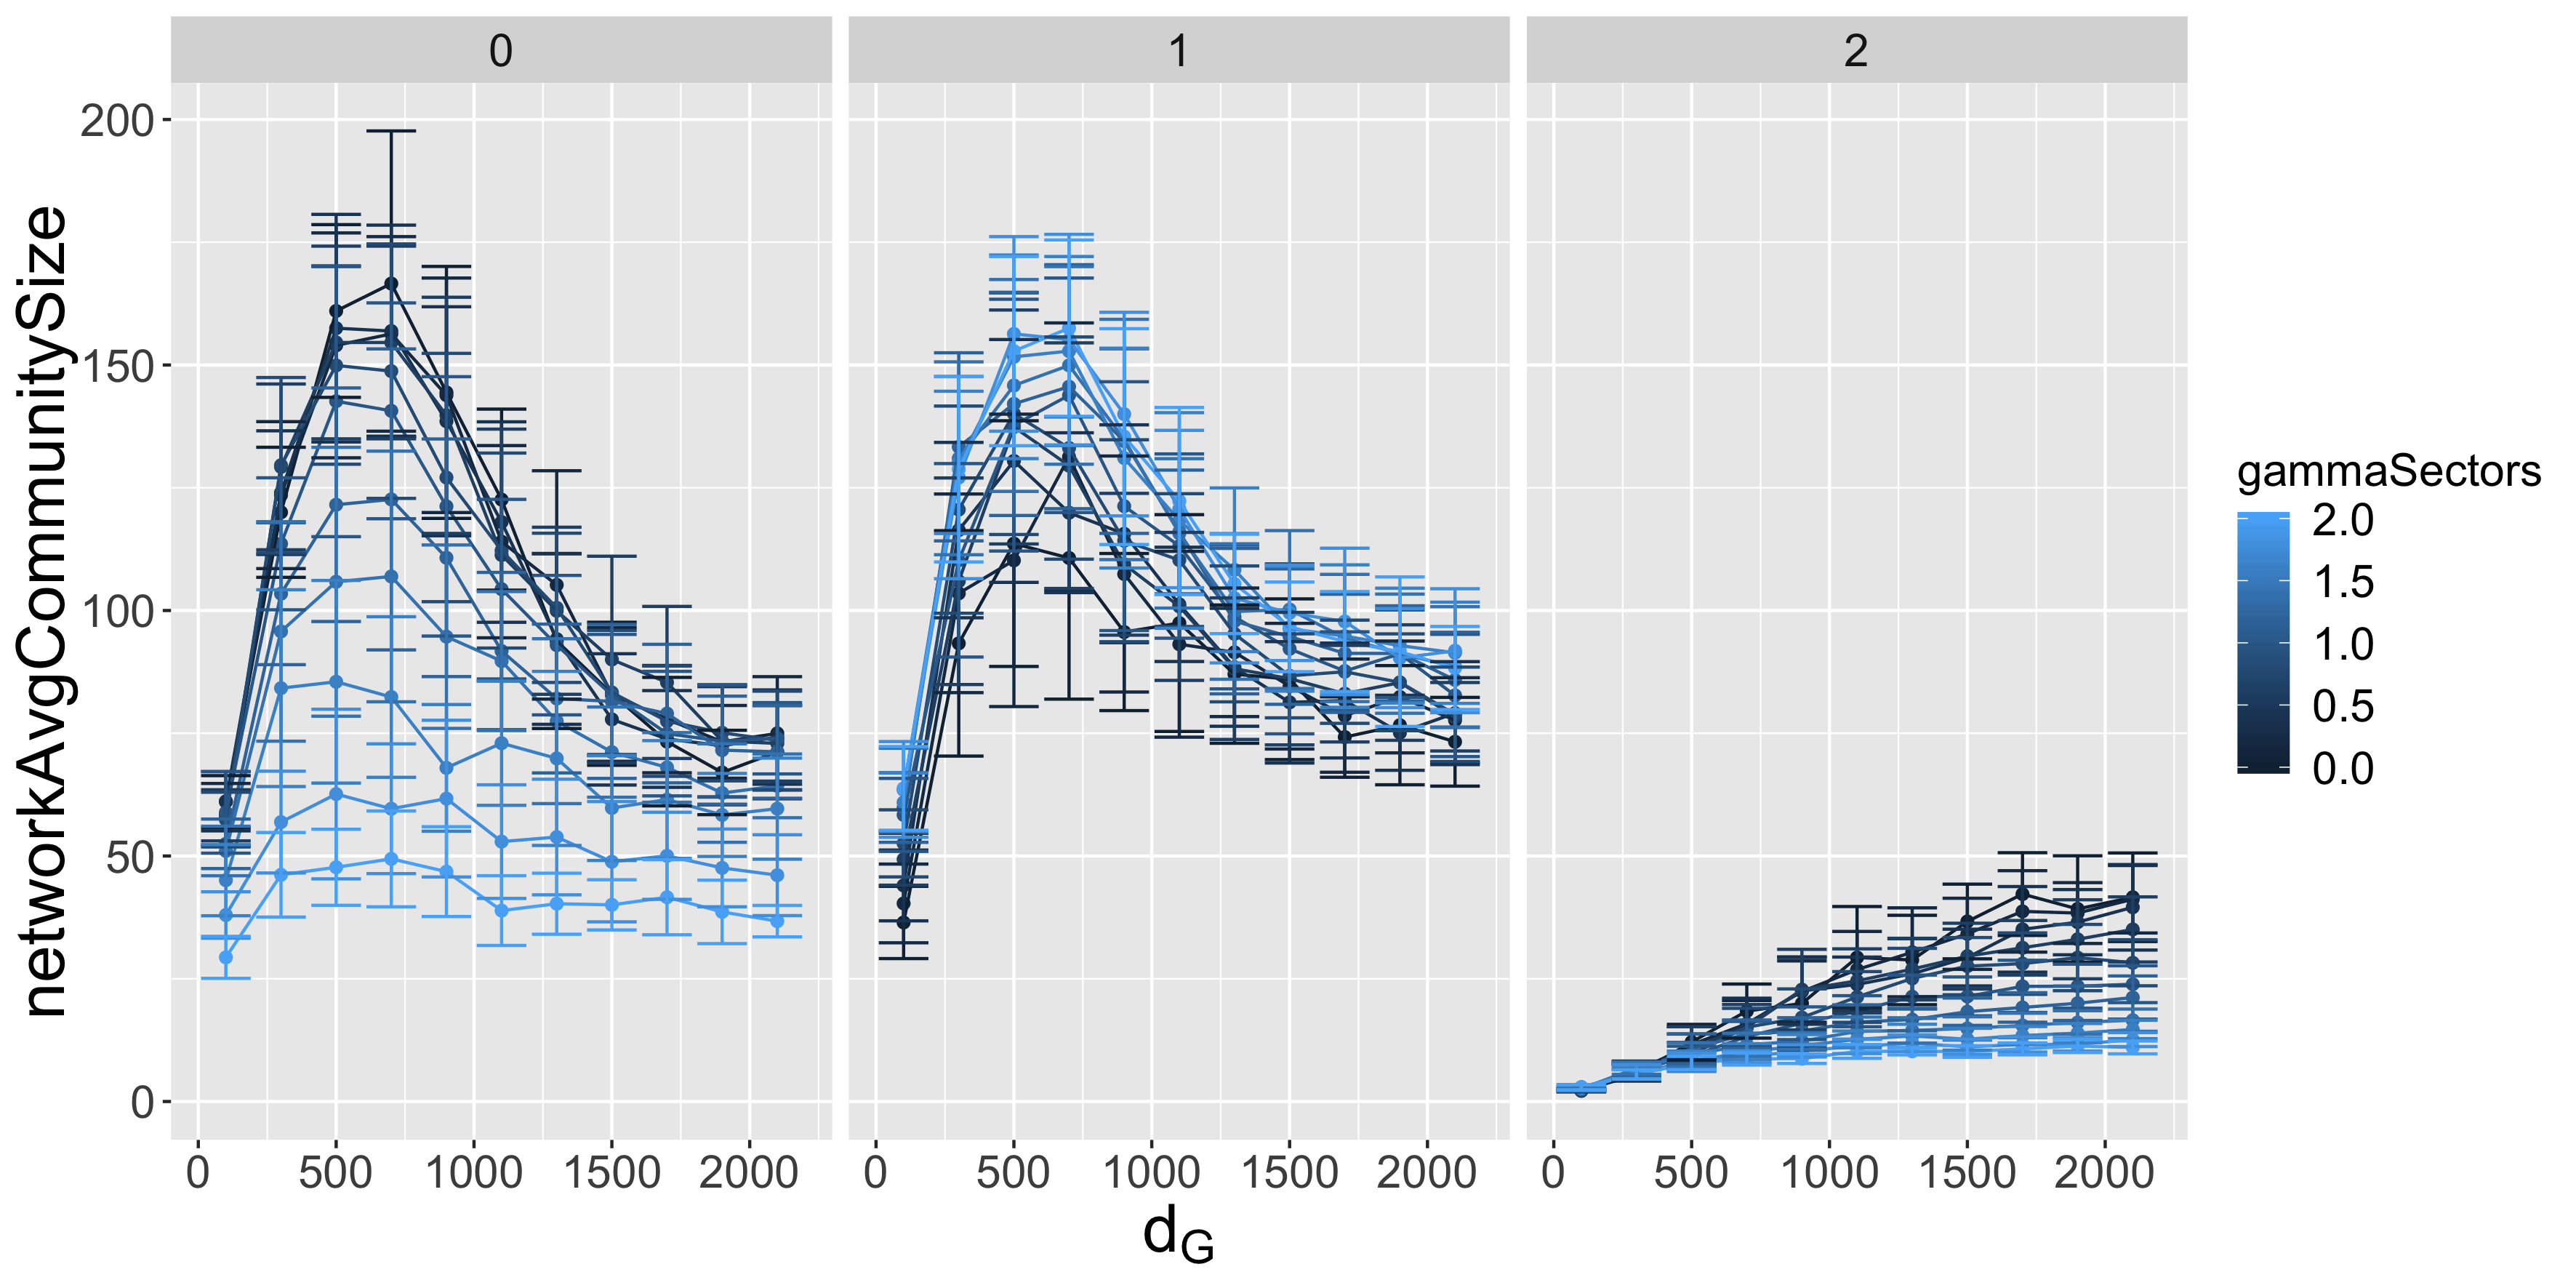
\includegraphics[width=\textwidth]{figures/networkAvgCommunitySize_countryGravityDecay2100_gammaDestination0_facetwrapgammaOrigin_colorgammaSectors.png}
}

% alors ici il faut reconnomer l'axe des ordonnees ca peut etre community size? qui est defini comment d'ailleurs ici? C'est la ou tu as dit que le pic aussi rapide est interessant, donc en si peu de temps la taille du reseaux grossi c'est ca :'(? et du coup comment expliquer le 2 a droite? 


%\sframe{Grid exploration}{
%    \centering
%
%    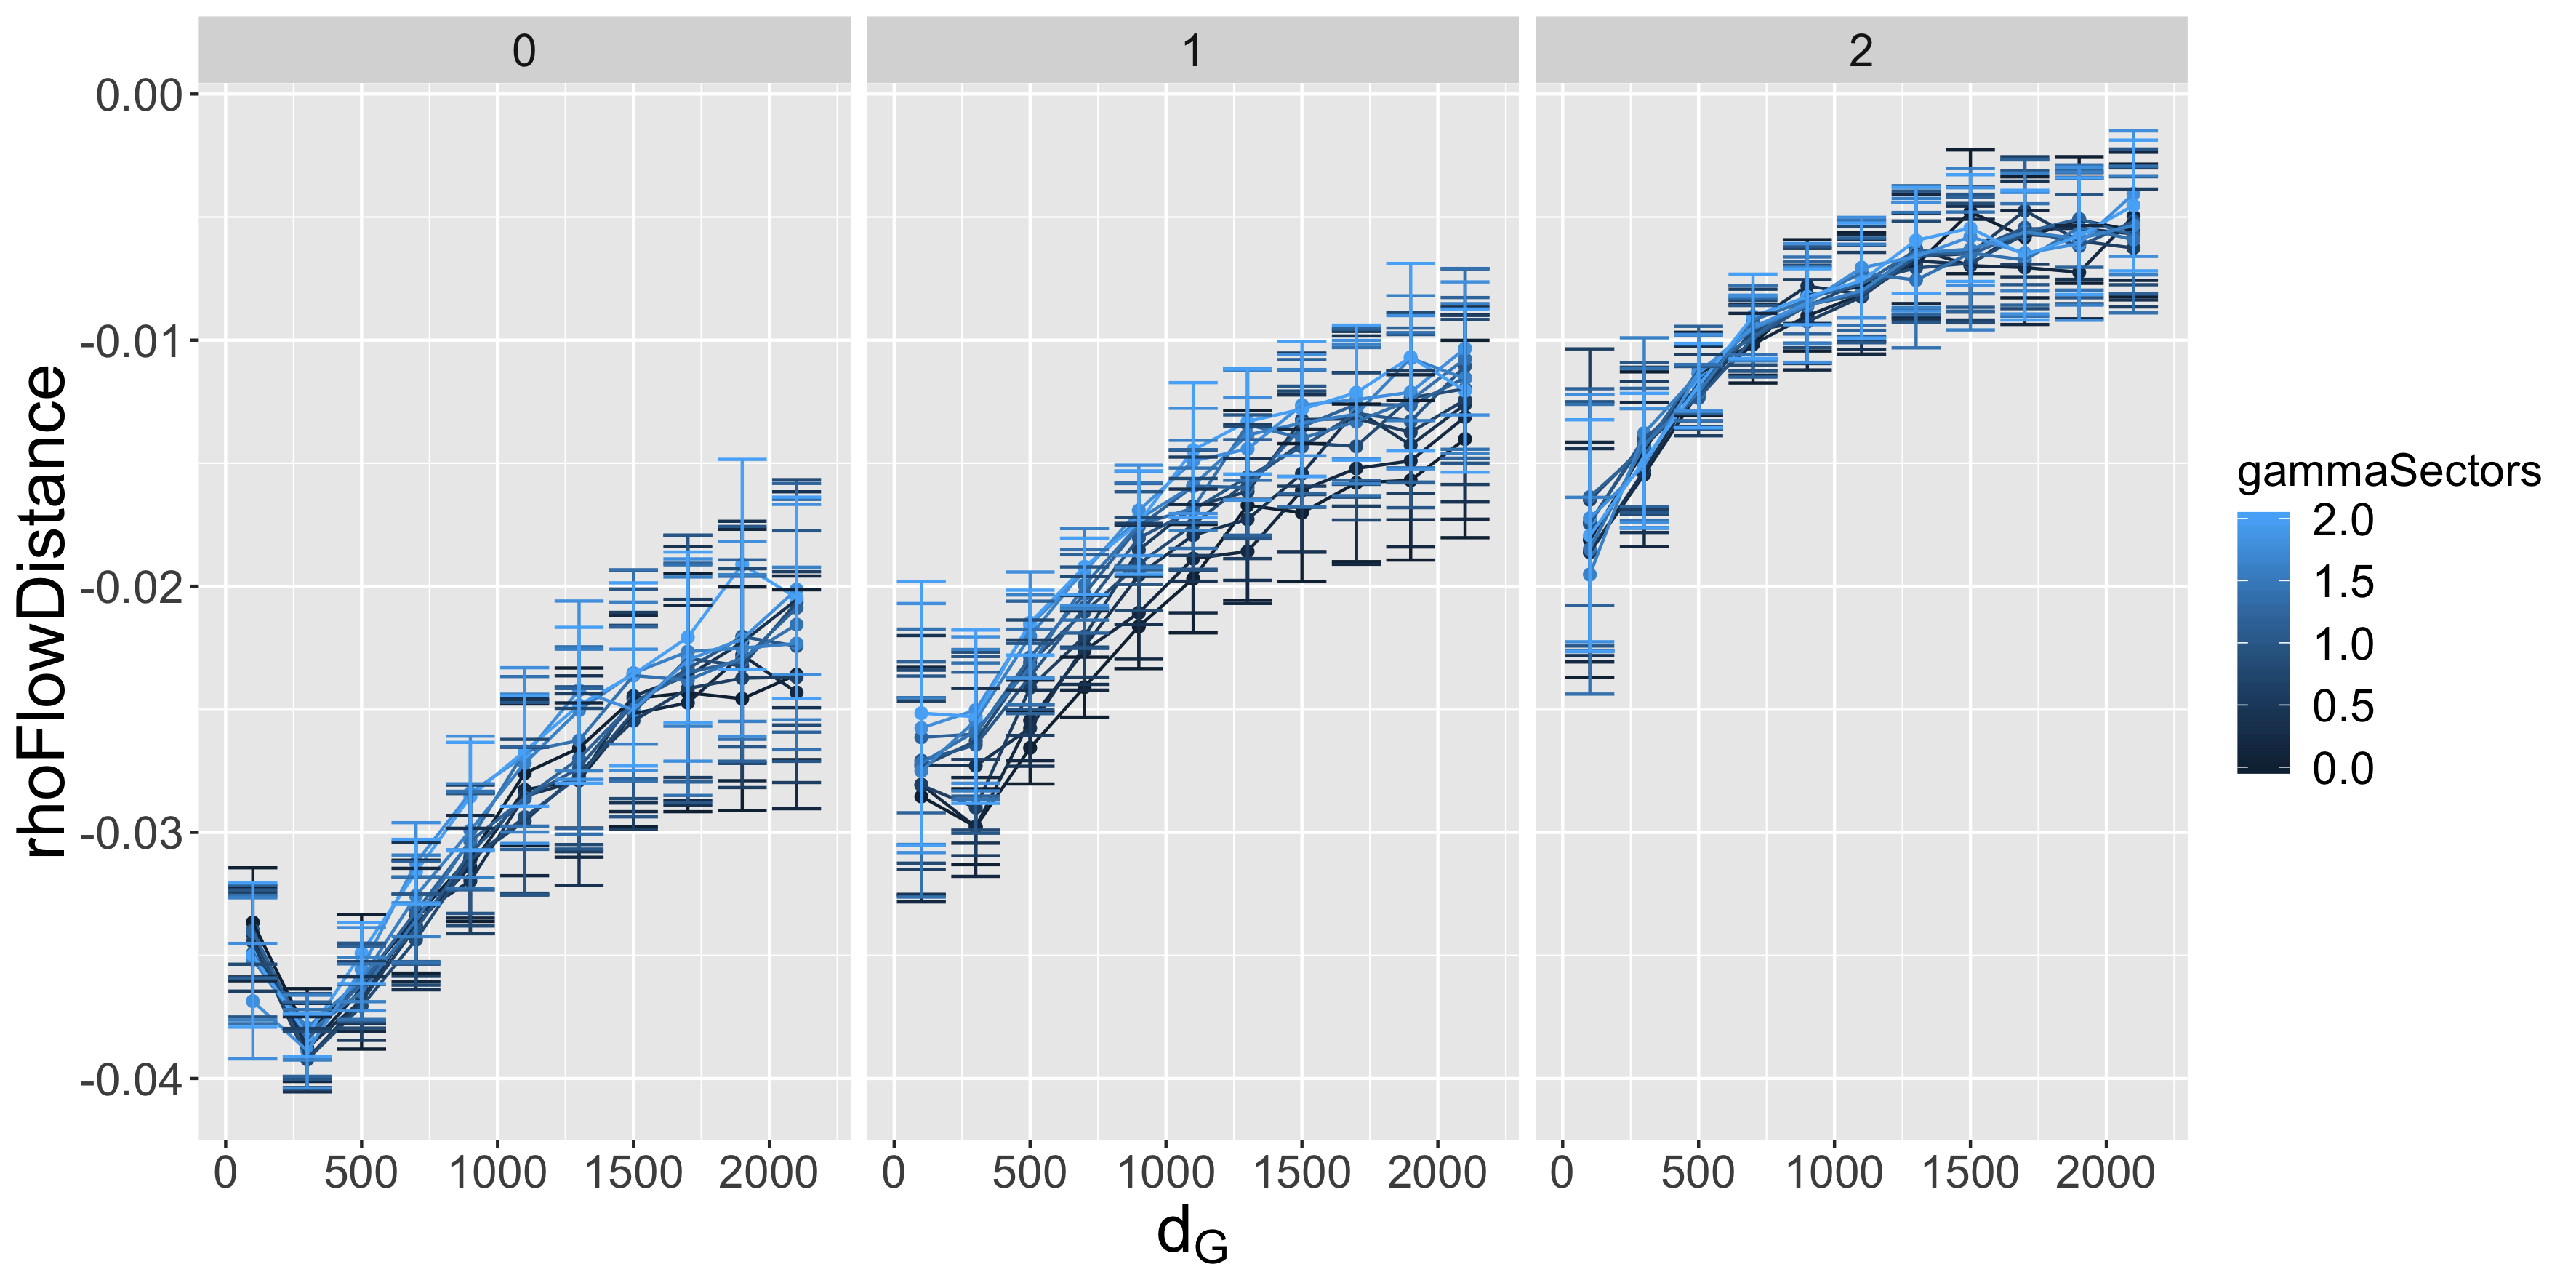
\includegraphics[width=\textwidth]{figures/rhoFlowDistance_countryGravityDecay2100_gammaDestination2_facetwrapgammaOrigin_colorgammaSectors.png}
%}

% idem la c'est pas facile a lire pour quelqu'un qui ne connait pas. c'est quoi rhoFlowDistance?
% le gamma sector c'est le parametre de la variable secteurs donc s? 
% en fait quand j'y pense pourquoi il yq u gradien du gamma et comment comprendre ces varations pour chqaue pqs de temps

% other experiments ? PSE on correlations ?




\section{Discussion}

% - future work etc (classical discussion)
% - on the role of model exploration and simulation to gain knowledge from the model

% further comparing with real data?

\sframe{On the role of model exploration}{

}


\sframe{Discussion}{

\textbf{Practical application}



\textbf{Developments}


}


\sframe{Conclusion}{

$\rightarrow$ A simulation model to understand processes of network emergence

$\rightarrow$ 


\bigskip
\bigskip


\textbf{Open repository for model and results at}

\texttt{https://github.com/JusteRaimbault/ABMCitiesFirms}

\textbf{Simulation data at}

\texttt{https://doi.org/10.7910/DVN/UPX23S}

\bigskip

\textbf{Acknowledgments}: thanks to the \textit{European Grid Infrastructure} for access to the infrastructure.


}



\sframe{Reserve slides}{

\centering

\Large

\textbf{Reserve Slides}

}



%%%%%%%%%%%%%%%%%%%%%
\begin{frame}[allowframebreaks]
\frametitle{References}
\bibliographystyle{apalike}
\bibliography{biblio}
\end{frame}
%%%%%%%%%%%%%%%%%%%%%%%%%%%%







\end{document}

